\documentclass[ 10pt]{beamer}

%\usepackage{beamerthemesplit}
\graphicspath{{Figures/}}
%\usetheme[height=1cm]{Rochester}
%\usetheme[height=1cm]{Singapore}
%\usetheme{Boadilla}
%\usetheme{boxes}
\usetheme[]{Boadilla} %secheader
%\useoutertheme[footline=authortitle,subsection=false,height=1cm]{miniframes}
%\useoutertheme[subsection=false,height=1cm]{smoothbars}

      %#make sure to change this part, since it is predefined
      %\defbeamertemplate*{footline}{infolines theme}
      \setbeamertemplate{footline}
        {
      \leavevmode%
      \hbox{%
      \begin{beamercolorbox}[wd=.333333\paperwidth,ht=2.25ex,dp=1ex,center]{author in head/foot}%
%        \usebeamerfont{author in head/foot}\insertshortauthor %~~(\insertshortinstitute)
        \usebeamerfont{author in head/foot}\insertshorttitle %~~(\insertshortinstitute)
      \end{beamercolorbox}%
      \begin{beamercolorbox}[wd=.333333\paperwidth,ht=2.25ex,dp=1ex,center]{title in head/foot}%
        \usebeamerfont{title in head/foot}\insertsection%: ~~ \insertsubsection
      \end{beamercolorbox}%
      \begin{beamercolorbox}[wd=.333333\paperwidth,ht=2.25ex,dp=1ex,right]{date in head/foot}%
        \usebeamerfont{date in head/foot}\insertshortdate{}\hspace*{2em}
        \insertframenumber{} / \inserttotalframenumber\hspace*{2ex} 

      \end{beamercolorbox}}%
      \vskip0pt%
    }
    
\usepackage{epic}
%\usepackage{natbib}
%\usepackage[notocbib]{apalike}

\usepackage{color}

\beamertemplatenavigationsymbolsempty
\usepackage{graphicx}
\usepackage{color}
\usepackage[mathscr]{eucal}
%\usepackage{subfig}
\usepackage{epsfig}
\usepackage[all]{xy}
\usepackage{url}
\usepackage{setspace}
%\usepackage{xmpmulti}
\DeclareMathOperator{\E}{E}
\DeclareMathOperator{\I}{I}
\DeclareMathOperator{\Var}{Var}
\DeclareMathOperator{\Cov}{Cov}
\DeclareMathOperator{\logit}{logit}
\DeclareMathOperator{\dom}{dom}
\DeclareMathOperator{\cl}{cl}
\DeclareMathOperator{\bd}{bd}
\DeclareMathOperator{\rbd}{rbd}
\DeclareMathOperator{\intr}{int}
\DeclareMathOperator{\rint}{rint}
\DeclareMathOperator{\con}{con}
\DeclareMathOperator{\pos}{pos}
\DeclareMathOperator{\aff}{aff}
\DeclareMathOperator{\epi}{epi}
\DeclareMathOperator{\lev}{lev}
\DeclareMathOperator{\spanl}{span}

\def\RR{{\mathbb R}}
\def\ZZ{{\mathbb Z}}
\def\DD{{\mathcal D}}
\def\XX{{\mathcal X}}
\def\YY{{\mathcal Y}}
\def\TT{{\mathcal T}}
\def\NN{{\mathcal N}}
\def\nubf{{\boldsymbol{\nu}}}
\def\etabf{{\boldsymbol{\eta}}}
\def\Zbf{{\boldsymbol{Z}}}
\def\gbf{{\boldsymbol{g}}}
\def\Ybf{{\boldsymbol{Y}}}
\newcommand{\deriv}[2]{\frac{d #1}{d #2}}
\newcommand{\dderiv}[2]{\frac{d^2 #1}{d #2^2}}
\newcommand{\pderiv}[2]{\frac{\partial #1}{\partial #2}}
\newcommand{\ppderiv}[2]{\frac{\partial^2 #1}{\partial #2^2}}
\newcommand{\ppmderiv}[3]{\frac{\partial^2 #1}{\partial #2 \partial #3}}
\newcommand{\fatdot}{\,\cdot\,}
\newcommand{\inner}[1]{\langle #1 \rangle}
\newcommand{\set}[1]{\{\, #1 \,\}}
\newcommand{\abs}[1]{\lvert #1 \rvert}
\newcommand{\norm}[1]{\lVert #1 \rVert}
\newcommand{\etaMLE}{\hat{\eta}_{\textrm{MLE}}}
\newcommand{\betaMLE}{\hat{\beta}_{\textrm{MLE}}}
\newcommand{\thetaLCM}{\hat{\theta}_{\textrm{LCM}}}
\newcommand{\etaLCM}{\hat{\eta}_{\textrm{LCM}}}
\newcommand{\yobs}{y_{\text{obs}}}
\newcommand{\Gammalim}{\Gamma_{\textrm{lim}}}
\newcommand{\CLCM}{C_{\textrm{LCM}}}

%\setbeamercovered{transparent}

\title{Parameter Estimation in Social Network Models}
\author{
  Saisuke Okabayashi 
%  Charles J. Geyer
}

\institute{Department of Statistics \\ University of Minnesota}

\date{April 5, 2011}


\begin{document}
%\usefoottemplate{\vbox{\tinycolouredline{structure!75}{\color{white}\textbf{\insertauthor\hfill}}\tinycolouredline{structure}{\color{white}\textbf{\inserttitle}\hfill}}}
\definecolor{darkblue}{rgb}{0,0.08,0.65}
\definecolor{darkblue}{rgb}{0,0.08,0.65}

\frame{\titlepage}
\section{Background: motivation}
\frame{
	\frametitle{My research is about}
\begin{itemize}
\item optimization
\item a modified curvature condition
%\item linear programming
%\item relative boundaries of convex hulls
\item limiting distributions of exponential families
%\item generic directions of recession
\end{itemize}
\vspace{0.4in}

%\pause
%\hspace{0.1in} \emph{\LARGE{\textcolor{orange}{But that's not how it began!} }}
}


\frame
{
  \frametitle{It began with some monks ...}
\begin{figure}
\begin{center} 
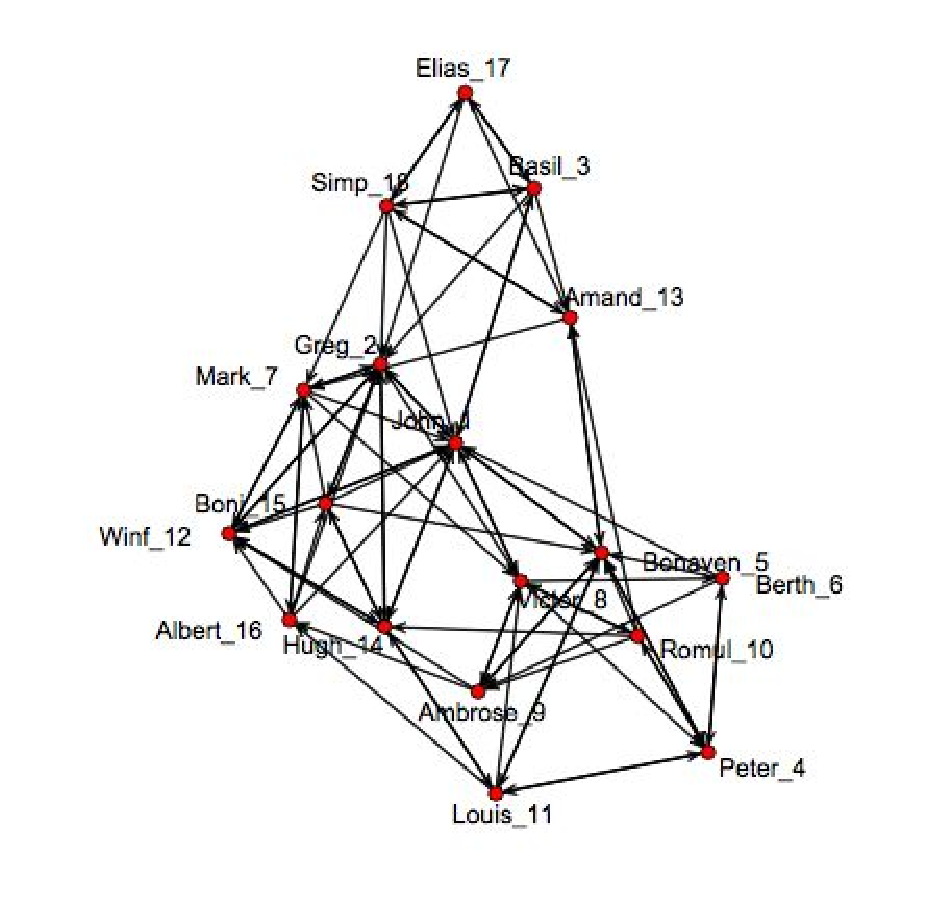
\includegraphics[height=2.7in]{samplike}
\caption{Sampson's (1969) affinity network among 18 monks in a monastery.  Data available in and plotted using \textcolor{darkblue}{\texttt{statnet}} package (Handcock et al, 2003) in R.} 
\end{center} 
\end{figure}
}
%\frame
%{
%  \frametitle{and... }
%
%\begin{figure}
%\begin{center} 
%\includegraphics[height=2.7in]{florentine}
%\caption{Padgett's (1994) Florentine marriage network among 16 Florentine families around 1430.} 
%\end{center} 
%\end{figure}
%}
\frame
{
  \frametitle{and... }
\begin{figure}
\begin{center} 
\includegraphics[height=2.55in]{fmh-gradesex2}
\caption{National Longitudinal Study of Adolescent Health friendship network of 1,461 students in grades 7 -- 12.  Squares = Boys, Circles = Girls.  

Sources: Resnick et al. (1997), Goodreau (2008).} 
\end{center} 
\label{fmh} 
\end{figure}
}
\frame
{
  \frametitle{and...}

\begin{figure}
\begin{center} 
\includegraphics[height=2.6in]{ecoli}
\caption{\textit{E. Coli} transcriptional regulation network.  
Nodes are operons, $i \to j$ indicates that $i$ encodes transcription factor that regulates $j$.

Sources: Shen-Orr et al. (2002), Hummel et al. (2009).} 
\end{center} 
\end{figure}
}

\frame
{
\frametitle{Why networks?}
{\large Networks are a conduit for \emph{flow}. } 
\vspace{2mm}

Flow can be:
\begin{itemize}
\item friendship
\item diseases
%\item needle-sharing
%\item money
\item data
%\item airplanes
\item commodities
\item trade
%\item ideas
%\item advice 
\item association (among terrorists)
\item binding (between proteins)
\item ...
\end{itemize}
\vspace{2mm}

\textcolor{darkblue}{Goal of a network model: explain the mechanism of this flow.} 
}

%%%%%%%%%%%%%%%%%%%%%%%%%%%%%%%%%%%%%%%%%%%%%%%%%%%%%%%%%%%%%
\section{Background: modeling networks}
\frame
{
\frametitle{A network, mathematically}
%\setbeamercovered{transparent}

A social network is a collection of \textcolor{darkblue}{actors} and 
\textcolor{darkblue}{relations} between each pair of actors.  
\vspace{1mm}

We can represent a network with $n$ actors as an $n \times n$ matrix $Y$, where
\begin{align*}
	Y_{ij} =
	\begin{cases} 	1 \quad \text{if a relation exists $i \to j$}\\
					0 \quad \text{otherwise}
	\end{cases}
\end{align*}

The Sampson monastery network:
{\tiny
\begin{table}[ht]
\begin{center}
\begin{tabular}{rrrrrrrrrrrrrrrrrr}
  \hline
0 & 1 & 1 & 0 & 1 & 0 & 1 & 0 & 0 & 0 & 1 & 0 & 0 & 0 & 1 & 0 & 0 & 0 \\ 
0 & 0 & 1 & 0 & 1 & 1 & 0 & 0 & 1 & 0 & 0 & 0 & 0 & 0 & 1 & 0 & 0 & 0 \\ 
0 & 1 & 0 & 0 & 0 & 0 & 1 & 1 & 0 & 0 & 0 & 0 & 0 & 1 & 0 & 0 & 0 & 0 \\ 
0 & 1 & 1 & 0 & 1 & 0 & 0 & 0 & 1 & 0 & 0 & 0 & 0 & 0 & 0 & 0 & 0 & 0 \\ 
1 & 1 & 0 & 1 & 0 & 1 & 0 & 0 & 0 & 0 & 0 & 0 & 0 & 0 & 0 & 0 & 0 & 0 \\ 
0 & 1 & 0 & 0 & 1 & 0 & 1 & 0 & 0 & 0 & 1 & 0 & 0 & 1 & 0 & 0 & 0 & 0 \\ 
1 & 0 & 1 & 1 & 1 & 0 & 0 & 0 & 1 & 1 & 0 & 0 & 0 & 0 & 0 & 0 & 0 & 0 \\ 
0 & 0 & 0 & 0 & 0 & 0 & 0 & 0 & 1 & 1 & 1 & 0 & 1 & 0 & 0 & 0 & 0 & 0 \\ 
0 & 1 & 0 & 0 & 0 & 0 & 1 & 1 & 0 & 1 & 1 & 0 & 0 & 0 & 0 & 1 & 0 & 0 \\ 
0 & 0 & 0 & 0 & 0 & 0 & 0 & 1 & 1 & 0 & 1 & 1 & 1 & 0 & 0 & 0 & 0 & 0 \\ 
0 & 0 & 0 & 0 & 0 & 1 & 0 & 1 & 1 & 1 & 0 & 1 & 0 & 0 & 0 & 0 & 0 & 0 \\ 
0 & 1 & 0 & 0 & 0 & 0 & 0 & 1 & 1 & 1 & 1 & 0 & 1 & 0 & 0 & 0 & 0 & 0 \\ 
0 & 0 & 0 & 0 & 0 & 0 & 1 & 1 & 1 & 1 & 0 & 0 & 0 & 1 & 0 & 0 & 0 & 0 \\ 
0 & 0 & 0 & 0 & 0 & 0 & 0 & 1 & 1 & 1 & 0 & 1 & 1 & 0 & 0 & 0 & 0 & 0 \\ 
0 & 1 & 0 & 0 & 0 & 0 & 0 & 0 & 0 & 0 & 0 & 0 & 1 & 0 & 0 & 0 & 0 & 1 \\ 
0 & 0 & 0 & 0 & 0 & 0 & 0 & 0 & 1 & 1 & 0 & 0 & 0 & 0 & 1 & 0 & 1 & 1 \\ 
0 & 0 & 0 & 0 & 0 & 0 & 0 & 0 & 0 & 1 & 0 & 0 & 0 & 0 & 1 & 1 & 0 & 1 \\ 
0 & 0 & 0 & 0 & 0 & 0 & 0 & 0 & 1 & 1 & 0 & 0 & 1 & 0 & 1 & 1 & 1 & 0 \\ 
   \hline
\end{tabular}
\end{center}
\end{table}}
}
%\frame
%{
%\frametitle{A network, mathematically}
%%\setbeamercovered{transparent}
%
%A social network is a collection of \textcolor{darkblue}{actors} and 
%\textcolor{darkblue}{relations} between each pair of actors.  
%\vspace{1mm}
%
%We can represent a network with $n$ actors as an $n \times n$ matrix $Y$, where
%\begin{align*}
%	Y_{ij} =
%	\begin{cases} 	1 \quad \text{if a relation exists $i \to j$}\\
%					0 \quad \text{otherwise}
%	\end{cases}
%\end{align*}
%
%The Sampson monastery network (directed):
%\only<1>{
%{\tiny
%\begin{table}[ht]
%\begin{center}
%\begin{tabular}{rrrrrrrrrrrrrrrrrr}
%  \hline
%0 & 1 & 1 & 0 & 1 & 0 & 1 & 0 & 0 & 0 & 1 & 0 & 0 & 0 & 1 & 0 & 0 & 0 \\ 
%0 & 0 & 1 & 0 & 1 & 1 & 0 & 0 & 1 & 0 & 0 & 0 & 0 & 0 & 1 & 0 & 0 & 0 \\ 
%0 & 1 & 0 & 0 & 0 & 0 & 1 & 1 & 0 & 0 & 0 & 0 & 0 & 1 & 0 & 0 & 0 & 0 \\ 
%0 & 1 & 1 & 0 & 1 & 0 & 0 & 0 & 1 & 0 & 0 & 0 & 0 & 0 & 0 & 0 & 0 & 0 \\ 
%1 & 1 & 0 & 1 & 0 & 1 & 0 & 0 & 0 & 0 & 0 & 0 & 0 & 0 & 0 & 0 & 0 & 0 \\ 
%0 & 1 & 0 & 0 & 1 & 0 & 1 & 0 & 0 & 0 & 1 & 0 & 0 & 1 & 0 & 0 & 0 & 0 \\ 
%1 & 0 & 1 & 1 & 1 & 0 & 0 & 0 & 1 & 1 & 0 & 0 & 0 & 0 & 0 & 0 & 0 & 0 \\ 
%0 & 0 & 0 & 0 & 0 & 0 & 0 & 0 & 1 & 1 & 1 & 0 & 1 & 0 & 0 & 0 & 0 & 0 \\ 
%0 & 1 & 0 & 0 & 0 & 0 & 1 & 1 & 0 & 1 & 1 & 0 & 0 & 0 & 0 & 1 & 0 & 0 \\ 
%0 & 0 & 0 & 0 & 0 & 0 & 0 & 1 & 1 & 0 & 1 & 1 & 1 & 0 & 0 & 0 & 0 & 0 \\ 
%0 & 0 & 0 & 0 & 0 & 1 & 0 & 1 & 1 & 1 & 0 & 1 & 0 & 0 & 0 & 0 & 0 & 0 \\ 
%0 & 1 & 0 & 0 & 0 & 0 & 0 & 1 & 1 & 1 & 1 & 0 & 1 & 0 & 0 & 0 & 0 & 0 \\ 
%0 & 0 & 0 & 0 & 0 & 0 & 1 & 1 & 1 & 1 & 0 & 0 & 0 & 1 & 0 & 0 & 0 & 0 \\ 
%0 & 0 & 0 & 0 & 0 & 0 & 0 & 1 & 1 & 1 & 0 & 1 & 1 & 0 & 0 & 0 & 0 & 0 \\ 
%0 & 1 & 0 & 0 & 0 & 0 & 0 & 0 & 0 & 0 & 0 & 0 & 1 & 0 & 0 & 0 & 0 & 1 \\ 
%0 & 0 & 0 & 0 & 0 & 0 & 0 & 0 & 1 & 1 & 0 & 0 & 0 & 0 & 1 & 0 & 1 & 1 \\ 
%0 & 0 & 0 & 0 & 0 & 0 & 0 & 0 & 0 & 1 & 0 & 0 & 0 & 0 & 1 & 1 & 0 & 1 \\ 
%0 & 0 & 0 & 0 & 0 & 0 & 0 & 0 & 1 & 1 & 0 & 0 & 1 & 0 & 1 & 1 & 1 & 0 \\ 
%   \hline
%\end{tabular}
%\end{center}
%\end{table}}
%}
%
%\uncover<2->{
%\begin{columns}[T]
%\begin{column}[T]{0.35\textwidth}
%\includegraphics[height=1.6in]{samplike-matrix}
%\end{column}
%
%\uncover<3->{
%\begin{column}[T]{0.65\textwidth}
%\vspace{5mm}
%
%$Y_{ij}$ are \alert{not} in general independent.
%\vspace{2mm}
%
%%This dependence is at the core of the ``network perspective'' in sociology.
%%\pause
%\begin{block}{\textbf{Our research}}
%Focus on models that capture dependency and \\
%find a method to fit them to data.
%\end{block}
%}
%\end{column}
%\end{columns}
%}
%
%}

\frame
{
\frametitle{01101010001 ...}
Take this matrix and represent entries with 0 as white, 1 as black.
\begin{columns}[T]
\begin{column}[T]{0.35\textwidth}
\includegraphics[height=1.6in]{samplike-matrix}
\end{column}
\pause
\begin{column}[T]{0.65\textwidth}
\vspace{5mm}

$Y_{ij}$ are \alert{not} in general independent.
\vspace{2mm}

%This dependence is at the core of the ``network perspective'' in sociology.
%\pause
\begin{block}{Our research}
Focus on models that capture dependency and \\
find a method to fit them to data.
\end{block}

\end{column}
\end{columns}
%\vspace{2mm}

%\textbf{Statistical inference:} determine what factors are important in shaping $Y$.
%global structure of relations.  
%\vspace{1mm}

%Factors may be actor specific: seniority or ethnicity.

%But we also want to include relational structures.


}
\section{Background: ERGM}
\frame
{
\frametitle{A network model}
\setbeamercovered{transparent}

%Writing down an expression for a network model is straightforward.  
%\vspace{2mm}

\textcolor{blue}{Exponential-family Random Graph Models (ERGM)} have log likelihood
\begin{align*}% \label{E:loglike}
	\ell( \eta) = \eta^T g(\yobs) - c(\eta)
\end{align*}
where 
\begin{itemize}
\item $\eta \in \RR^d$ is a \textcolor{blue}{natural parameter} vector
\vspace{1mm}
\item $g(y)\in\RR^d$ is a \textcolor{blue}{natural statistic} vector of the \emph{observed network} $\yobs \in \YY$
\vspace{1mm}
%\item $\YY$ is the space of all possible networks for a fixed number of actors
%\vspace{1mm}
\item $	c(\eta) = \log \sum_{x \in \YY} e^{\eta^T g(x)}$, is the log of the 
\textcolor{blue}{normalizing constant}.
\end{itemize}




}

\frame
{
\frametitle{How to include dependency}
The natural statistic $g(y)$ is a vector of \textcolor{darkblue}{network statistics} of interest.  
\vspace{3mm}

Some examples (for an undirected network):
\begin{itemize}
	\item number of edges, $\sum_{i<j} Y_{ij}$
	\item number of triangles, $\sum_{i < j < k} Y_{ij}Y_{jk}Y_{ki}$
\end{itemize}
\vspace{2mm}

So, in this case,
\begin{align*}
	g(y) = \left( \sum_{i<j} Y_{ij}, 
					\sum_{i < j < k} Y_{ij}Y_{jk}Y_{ki} \right ).
\end{align*}
%\emph{That's it!}
\vspace{1mm}

\pause
\begin{alertblock}{Issue}
Sum in $c(\eta)$ is over all $\YY$, which can be an astronomical number of graphs.
\vspace{1mm}

$\implies$ Don't evaluate the log likelihood $\ell(\eta)$.

\vspace{3mm}

%\pause
\textcolor{blue}{How can you do parameter estimation---find MLEs---if \emph{you can't 
evaluate $\ell(\eta)$?} }
\end{alertblock}
}

%
%\frame
%{
%\frametitle{Number of graphs in $\YY$}
%%\setbeamercovered{transparent}
%\begin{table}[h] 
%%\caption{Sample space size for undirected networks with different number of 
%%actors.}
%
%\begin{tabular}{ccl} 
%\hline 
%Nodes & Possible Edges & Total Graphs \\ [1ex]
%\hline
%5 & ${5 \choose 2} = 10$ & $2^{10} = 1024$ \\ [1ex]
%6 & ${6 \choose 2} = 15$ & $2^{15} = 32,768$ \\ [1ex]
%7 & ${7 \choose 2} = 21$ & $2^{21} = 2,097,152$ \\ [1ex]
%8 & ${8 \choose 2} = 28$ & $2^{28} = 268,435,456$ \\ [1ex]
%9 & ${9 \choose 2} = 36$ & $2^{36} = 68,719,476,736$ \\ [1ex]
%10 & ${10 \choose 2} = 45$ & $2^{45} = 3.518437\times10^{13}$ \\ [1ex]
%\hline 
%\end{tabular} \label{T:number graphs}
%\end{table}
%\pause
%
%%The sum in $c(\eta)$ is over an astronomical number of terms for 
%%even moderate sized networks.
%\vspace{1mm}
%
%$\implies$ Don't evaluate the log likelihood function, $\ell(\eta)$.
%
%\vspace{3mm}
%
%\pause
%\textcolor{blue}{How can you do parameter estimation---find MLEs---if \emph{you can't 
%evaluate $\ell(\eta)$?} }
%}

%%%%%%%%%%%%%%%%%%%%%%%%%%%%%%%%%%%%%%%%%%%%%%%%%%%%%%%%%%%%%
%\section{Parameter estimation}
%\frame
%{
%\frametitle{Parameter estimation}
%We have a model. Let's fit it to an observed network, $\yobs$.
%\vspace{3mm}
%
%What is the value for $\eta$ such that the model assigns the highest probability to the observed data?
%\vspace{2mm}
%
%Maximum likelihood estimator (MLE)!
%\vspace{10mm}
%
%\pause
%\large But how do you find $\eta$ that maximizes $\ell(\eta)$ if \emph{you can't 
%evaluate $\ell(\eta)$?}
%}

%\frame
%{
%\frametitle{Methods that are out there}
%\begin{columns}[]
%\begin{column}[T]{0.6\textwidth}
%\includegraphics[height=2.8in]{mck-final.pdf}
%%\caption{Adolescent Health.} 
%\end{column}
%\begin{column}[t]{0.4\textwidth}
%{\small
%Overall satisfaction
%\vspace{1mm}
%
%\includegraphics[height=0.13in]{CR5.pdf} $\quad$ very good\\
%\vspace{1mm}
%\includegraphics[height=0.13in]{CR4.pdf} $\quad$ good\\
%\vspace{1mm}
%\includegraphics[height=0.13in]{CR3.pdf} $\quad$ neutral\\
%\vspace{1mm}
%\includegraphics[height=0.13in]{CR2.pdf} $\quad$ bad\\
%\vspace{1mm}
%\includegraphics[height=0.13in]{CR1.pdf} $\quad$ very bad\\
%\vspace{2mm}
%}
%%{\scriptsize
%%\textbf{MCMC-MLE} = Markov chain Monte Carlo Maximum Likelihood Estimator (Geyer and Thompson, 1992)\\
%%\vspace{1mm}
%%\textbf{Steplength MCMC-MLE} = Hummel et al. (2010)\\
%%\vspace{1mm}
%%\textbf{SA} = stochastic approximation \\
%%\vspace{1mm}
%%\textbf{MPLE} = Maximum pseudolikelihood estimator
%%}
%
%\end{column}
%\end{columns}
%}
\section{Parameter estimation}
\frame
{
\frametitle{Methods for parameter estimation}
\begin{columns}[]
\begin{column}[T]{0.6\textwidth}
\includegraphics<1>[height=2.8in]{mck-final-bare.pdf}
\includegraphics<2>[height=2.8in]{mck-final.pdf}
\includegraphics<3->[height=2.8in]{mck-final-overlay.pdf}
%\caption{Adolescent Health.} 
\end{column}
\begin{column}[t]{0.4\textwidth}
{\small
Overall satisfaction

\vspace{1mm}
\includegraphics[height=0.13in]{CR5.pdf} $\quad$ very good\\
\vspace{1mm}
\includegraphics[height=0.13in]{CR4.pdf} $\quad$ good\\
\vspace{1mm}
\includegraphics[height=0.13in]{CR3.pdf} $\quad$ neutral\\
\vspace{1mm}
\includegraphics[height=0.13in]{CR2.pdf} $\quad$ bad\\
\vspace{1mm}
\includegraphics[height=0.13in]{CR1.pdf} $\quad$ very bad\\
\vspace{1mm}
}

\uncover<3->{\small
\begin{block}{Our approach}
\begin{itemize}
\item Use iterated estimates
\begin{align*}
	\eta_{k+1} = \eta_k + \alpha_k p_k
\end{align*}
\item Don't evaluate $\ell( \eta)$
\vspace{1mm}

\item Don't use $\nabla^2 \ell( \eta)$
%\begin{itemize}
%	\item Can be expensive
%	\item May be near singular
%\end{itemize}
\end{itemize}
\end{block}
}
\end{column}
\end{columns}

}
%\frame
%{
%\frametitle{Methods that are out there}
%\begin{figure}
%\begin{center} 
%\includegraphics[height=3in]{mck-after.png}
%%\caption{Adolescent Health.} 
%\end{center} 
%\end{figure}
%}
%%%%%%%%%%%%%%%%%%%%%%%%%%%%%%%%%%%%%%%%%%%%%%%%%%%%%%%%%%%%%%

%\frame
%{
%\frametitle{Designing an algorithm: wish list}
%%\setbeamercovered{transparent}
%
%Our algorithm should
%\begin{itemize}
%\item Converge to the MLE $\etaMLE$, if it exists.
%\item Work from \emph{any} starting point $\eta_0$.
%\item No trial-and-error calibration.
%%\item In short, we want \includegraphics[height=0.13in]{CR5.png}
%\end{itemize}
%\vspace{3mm}
%
%\pause
%This means:
%\begin{itemize}
%\item Don't evaluate log likelihood function $\ell( \eta)$
%\vspace{1mm}
%
%\item Don't use second derivative of log likelihood $\nabla^2 \ell( \eta)$
%\begin{itemize}
%	\item Can be expensive to compute
%	\item May be near singular when $\eta_k$ is far from solution
%\end{itemize}
%\end{itemize}
%
%\textbf{Keep it simple!} %\pause \textbf{(stupid)}
%}

\section{Algorithm: intuition}
\frame
{
\frametitle{So what \emph{do} we have??}
\setbeamercovered{transparent}

We have the  {\textcolor{blue}{\emph{gradient}, $\nabla \ell(\eta)$.} }
%\vspace*{2mm}
For exponential families,
\begin{align*}
	\nabla \ell( \eta ) &= g(y_{obs}) - \E_{\eta} g(Y) 
	\uncover<2->{ \approx  g(y_{obs}) -  \frac{1}{m}\sum_{i = 1}^m g(Y_i) }
\end{align*}

%\pause
%We can approximate
%When $E_\eta g(Y)$ cannot be calculated exactly, %it can be well-approximated by
%\begin{align*}
%E_\eta g(Y) \approx \frac{1}{m}\sum_{i = 1}^m g(Y_i)
%\end{align*}
\uncover<2->{
where $Y_1$, $\ldots$, $Y_m$ are an MCMC sample from distribution with parameter $\eta$. }
\vspace*{7mm}

\uncover<3->{

\begin{block}{Using gradient in algorithm updates}
\begin{columns}[]
\begin{column}[t]{0.32\textwidth}
%\textcolor{darkblue}{iterated estimates}
%Iterated estimates:
\begin{align*}
	\eta_{k+1} = \eta_k + \alpha_k p_k
\end{align*}
$\alpha_k =$ scalar \textcolor{black}{step size}\\
$p_k = $ \textcolor{black}{search direction} %that is an ascent direction of $\ell(\eta)$
%\vspace*{2mm}
\end{column}

%\uncover<3->{
\begin{column}[t]{0.63\textwidth}
%Use gradient:
\begin{itemize}
\item \textcolor{blue}{$\nabla \ell(\eta_k) = 0$} $\implies$ found MLE
\vspace*{2mm}
\item Make $p_k$ an ascent direction, possibly \textcolor{blue}{$\nabla\ell(\eta_k)$}
\vspace*{2mm}
\item \textcolor{blue}{Choose $\alpha_k$ that guarantees convergence}
%\item Ensure adequate progress  in each step  (pick $\alpha_k$)
%\vspace*{2mm}
\end{itemize}
\end{column}
\end{columns}
\end{block}
}
}

%\frame
%{
%\frametitle{Framework for our algorithm}
%\setbeamercovered{transparent}
%Use iterated estimates
%\begin{align*}
%	\eta_{k+1} = \eta_k + \alpha_k p_k
%\end{align*}
%where $\alpha_k$ is a \textbf{step size} and  $p_k$ is a \textbf{search direction} that
%is an \emph{ascent direction} of the log likelihood.
%\vspace{3mm}
%
%\pause
%\begin{itemize}
%\item Taking steps in an ascent direction gets us progress towards maximum, but does not guarantee \emph{sufficient} progress.
%\vspace{3mm}
%
%\item Need a way to choose good step sizes to guarantee \emph{convergence} to maximum.
%\end{itemize}
%
%}

\frame
{
  \frametitle{Curvature condition}
%\begin{columns}[]
%%\begin{column}[t]{0.35\textwidth}
%{
%Iterated estimates
%\begin{align*}
%	\eta_{k+1} = \eta_k + \alpha_k p_k
%\end{align*}
%
%$\alpha_k =$ \emph{step size}\\
%$p_k = $ \emph{search direction} that
%is an ascent direction of $\ell(\eta)$
%\vspace{10mm}
%
%\textcolor{blue}{\emph{How to choose $\alpha_k$?}}
%}
%\end{column}
%
%\begin{column}[T]{0.65\textwidth}
%{
%\pause

%\textcolor{darkblue}{Curvature condition}
%\vspace{1mm}

Find $\alpha_k$ that satisfies
\begin{align*}
	 0 & \leq \nabla \ell( \eta_k + \alpha_k p_k)^T p_k \leq c \nabla \ell(\eta_k)^T 
p_k
\end{align*}
%}
for some $0 < c < 1$.
\vspace{2mm}

    \scalebox{.28}{\input{Figures/alphamax.pdf_t}}
%\end{column}
%\end{columns}
}

%\frame
%{
%  \frametitle{Curvature condition}
%Find an $\alpha_k$ that satisfies
%\begin{align*}
%	 0 & \leq \nabla \ell( \eta_k + \alpha_k p_k)^T p_k \leq c \nabla \ell(\eta_k)^T 
%p_k
%\end{align*}
%\begin{figure}[h]
%\centering
%    \scalebox{.25}{\input{Figures/alphamax.pdf_t}}
%	\caption{Acceptable region for step size $\alpha_k$ along a search direction $p_k$.}
%\label{F:alpha_region}
%\end{figure}
%}



\section{Algorithm: theory}

\frame
{
\frametitle{Results}
{\small
%\begin{block}{Assumptions}
%a regular exponential family on a finite sample space 
%$p_k$ is a descent direction.
%\end{block}

\begin{theorem}[Exponential family zero gradient attainment] \label{Thm:log like max}
Consider any line search of the form 
\begin{align}
	\eta_{k+1} &= \eta_k + \alpha_k p_k \label{E:eta_update}
\end{align}
used to minimize $-\ell(\fatdot)$. %such that the angle $\theta_k$ between the search direction $p_k$ and steepest descent 
%direction $-\nabla \ell(\eta_k)$ is 
%restricted to be less than 90 degrees by
%\begin{align*}
%\cos \theta_k \geq \delta > 0
%\end{align*}
% for some fixed $\delta > 0$.  
Then it is possible to find an $\alpha_k$ that satisfies %the \emph{curvature condition}
\begin{align}
	0 \leq \nabla \ell( \eta_k + \alpha_k p_k)^T p_k  \leq c \nabla \ell(\eta_k)^T p_k  
\label{E:Wolfe-ll}
\end{align}
for some fixed $0 < c < 1$.
Repeated iterations of \eqref{E:eta_update} along a descent direction 
satisfying \eqref{E:Wolfe-ll} will produce a sequence, $\eta_1, \eta_2, \ldots$ such 
that
\begin{align*}
	\lim_{k \to \infty} \lVert \nabla \ell(\eta_k) \rVert = 0.
\end{align*}
\end{theorem}
\vspace{2mm}

\begin{theorem}[MLE convergence] \label{Thm:Line Search works}
When the MLE exists, the 
line search starting at any $\eta_0$ will converge to $\etaMLE$.
\end{theorem}
}

}
%
%\frame
%{
%\frametitle{MLE attainment}
%Previous theorem $\implies$ our algorithm gets us 
%$\lVert \nabla \ell(\eta_k) \rVert \to 0$.  
%\vspace{2mm}
%
%
%\vspace{2mm}
%
%\begin{theorem}[MLE convergence] \label{Thm:Line Search works}
%For a regular exponential family with minimal representation where the MLE exists, the 
%line search described in 
%previous theorem can be applied to $-\ell(\eta)$ so that a search 
%starting at any $\eta_0$ will converge to $\etaMLE$.
%\end{theorem}
%
%}

%%%%%%%%%%%%%%%%%%%%%%%%%%%%%%%%%%%%%%%%%%%%%%%%%%%%%%%%%%%%%
\section{Examples: monks}
\frame
{
  \frametitle{Toy example: Monks}  
  \setbeamercovered{transparent}

\begin{columns}[t]
\begin{column}[T]{0.3\textwidth}
%\includegraphics[height=1.5in]{g9-basic}
%\pgfputat{\pgfxy(0,0)}{\pgfbox[left,top]{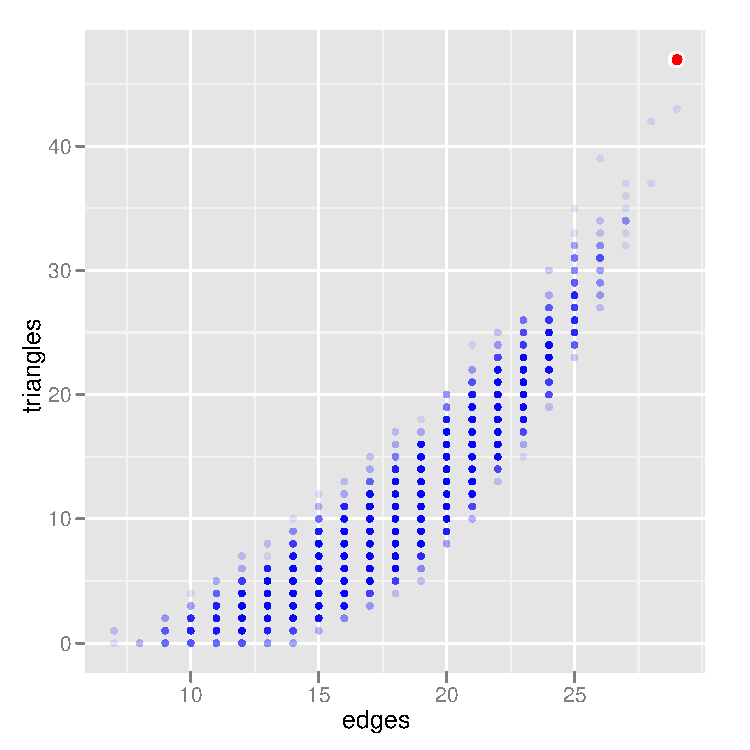
\includegraphics[width=\textwidth]{MCsample-bare} }}
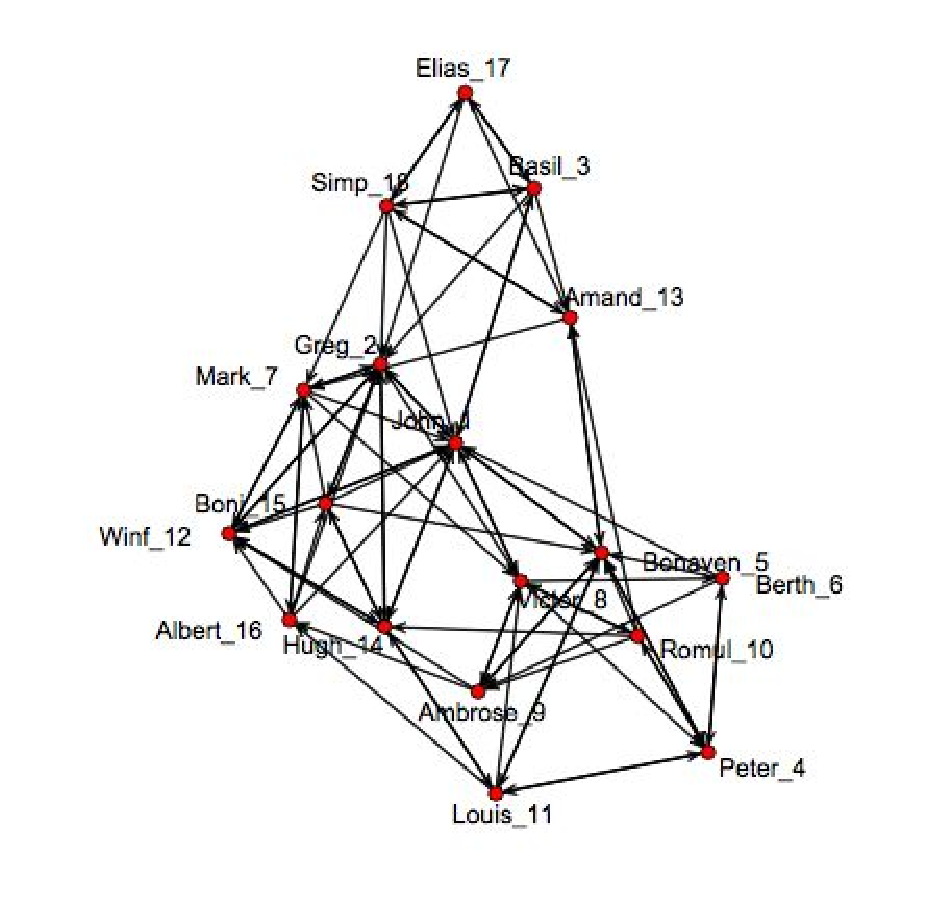
\includegraphics[width=1.5in]{samplike}
\end{column}

\begin{column}[r]{0.7\textwidth}
Use a simple model with $g(y) =$ (\# of edges):
%MLE can be found analytically,
\begin{align*}
	\etaMLE = -0.9072.
\end{align*}

%\pause
%\textcolor{darkblue}{MCMC-MLE:} %struggles when $\eta_0$ is far from $\etaMLE$.
%\vspace{2mm}

Use $\eta_0 = 1$, which is considered ``far" for MCMC-MLE.%took 10 iterations to converge.
%(default max iteration in \texttt{statnet} package is 3).
\end{column}
\end{columns}

%\pause
%We ran our algorithm starting at same $\eta_0=1$.  
Our algorithm converged after 21 iterations with 5 parameter updates.
{\footnotesize
\begin{table}
\begin{center}
\begin{tabular}{rrrrrrlrr}
  \hline
    &  &  &  & \multicolumn{1}{c}{inner}\\
  \multicolumn{1}{c}{$k$} & 
  \multicolumn{1}{c}{$\eta_k$} &
  \multicolumn{1}{c}{$\lVert \nabla \ell(\eta_k) \rVert$} &
  \multicolumn{1}{c}{$\alpha_k$} &
  \multicolumn{1}{c}{loop }\\
    &  &  &  & \multicolumn{1}{c}{count}\\
  \hline
   0 &  $1.0000$ & 135.64 &  0.012 & 8\\
   1 & $-0.6649$ & 15.99  &  0.014 & 2 \\
   2 & $-0.8817$ & 1.57   &  0.014 & 3 \\
   3 & $-0.9043$ & 0.22   &  0.012 & 8 \\
   4 & $-0.9069$ & 0.03   &  &  \\
   \hline
\end{tabular} \label{T:Sampson redo}
\end{center}
\end{table}}
}

\section{Examples: high school friendship}

\frame
{
  \frametitle{Example: large(ish) friendship network---1461 actors}  
 \setbeamercovered{transparent}
\begin{columns}[t]
\begin{column}[T]{0.3\textwidth}
%\includegraphics[height=1.5in]{g9-basic}
%\pgfputat{\pgfxy(0,0)}{\pgfbox[left,top]{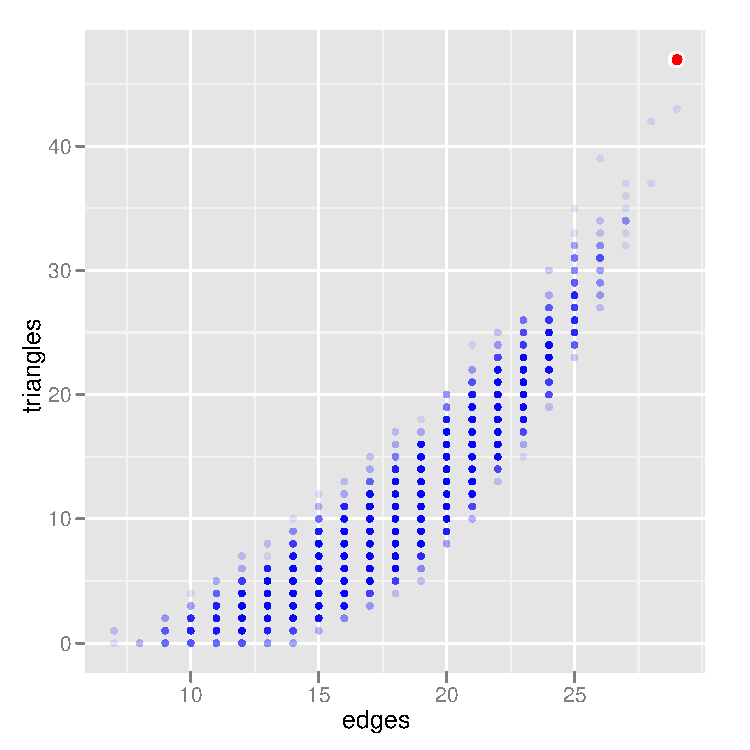
\includegraphics[width=\textwidth]{MCsample-bare} }}
\includegraphics[width=1.45in]{fmh-gradesex2}
\end{column}

\begin{column}[T]{0.7\textwidth}
A more realistic model with $g(y)$ including terms for
% \textbf{actor specific attributes} in addition to \textbf{network structures}.  
\vspace{1mm}
\begin{itemize}
\item Grade, Race, Sex
\vspace{1mm}

\item Edges, GWESP
\vspace{5mm}
\end{itemize}
%\pause

\textcolor{darkblue}{MCMC-MLE:}  \hspace{1mm} $\eta_0 = $ MPLE, very close to MLE

\textcolor{darkblue}{Our algorithm:} $\eta_0 = (0,0,0,0,0)$
\end{column}
\end{columns}
\vspace{5mm}

%\pause
Stopped our algorithm after 22 updates over 148 iterations, taking 1hr 40min.
\begin{table}
\begin{center} 
\begin{tabular}{rrrrrr}
  \hline
 & edges & Grade & Race & Sex & GWESP \\ 
  \hline
$\hat{\eta}_{\textrm{MCMCMLE}}$ & $-9.790$ & 2.755 & 0.906 & 0.780 & 1.813 \\ 
$\hat{\eta}_{\textrm{linesearch}}$ & 	$-9.893$	&	2.81	&	0.943	&	0.794	&	1.814\\ 
   \hline
\end{tabular}\label{T:FauxMagnolia}
\end{center}
\end{table}
}


\frame{
\frametitle{Algorithm summary}
{\scriptsize
\begin{table}
\begin{center} 
\begin{tabular}{rrrrrrr}
  \hline
  &  &  &  &  &  & \multicolumn{1}{c}{inner}\\
  \multicolumn{1}{c}{$k$} & 
  \multicolumn{1}{c}{$\eta[1]$} &
  \multicolumn{1}{c}{$\eta[2]$} &
  \multicolumn{1}{c}{$\eta[3]$} &
  \multicolumn{1}{c}{$\eta[4]$} &
  \multicolumn{1}{c}{$\eta[5]$} &
  \multicolumn{1}{c}{loop }\\
  &  & &  &  &  & \multicolumn{1}{c}{count}\\
\hline
0&	0& 0&	0&	0&	0 & - \\% &	89678.2 \\
1	&	-4.775	&	-0.824	&	-2.65	&	-2.384	&	-5.605	& 39	\\
2	&	-8.159	&	1.061	&	-0.847	&	-0.89	&	-4.519	& 1	\\
3	&	-7.35	&	1.836	&	-0.101	&	-0.234	&	-4.135	& 4	\\
4	&	-7.679	&	2.308	&	0.381	&	0.255	&	-3.225	& 3	\\
5	&	-7.933	&	2.185	&	0.263	&	0.155	&	-3.111	& 2	\\
6	&	-9.812	&	3.076	&	1.142	&	1.002	&	1.078	& 19	\\
...\\
%7	&	-9.887	&	3.011	&	1.078	&	0.939	&	1.098	& 5	\\
%8	&	-9.913	&	3.007	&	1.065	&	0.888	&	1.494	& 2	\\
%9	&	-9.944	&	2.978	&	1.037	&	0.862	&	1.488	& 4	\\
%10	&	-9.992	&	2.915	&	0.982	&	0.79		&	1.73		& 2	\\
%11	&	-9.984	&	2.92		&	0.988	&	0.795	&	1.737	& 4	\\
%12	&	-9.981	&	2.92		&	0.989	&	0.796	&	1.741	& 6	\\
%13	&	-9.966	&	2.903	&	0.983	&	0.796	&	1.768	& 5	\\
%14	&	-9.969	&	2.898	&	0.979	&	0.793	&	1.766	& 4	\\
%15	&	-9.896	&	2.813	&	0.946	&	0.796	&	1.821	& 5	\\
%16	&	-9.898	&	2.811	&	0.944	&	0.794	&	1.819	& 4	\\
%17	&	-9.896	&	2.811	&	0.944	&	0.795	&	1.818	& 5	\\
%18	&	-9.896	&	2.81		&	0.943	&	0.794	&	1.816	& 2	\\
%19	&	-9.895	&	2.81		&	0.944	&	0.794	&	1.817	& 3	\\
%20	&	-9.895	&	2.81		&	0.943	&	0.794	&	1.816	& 9	\\
%21	&	-9.894	&	2.81		&	0.944	&	0.794	&	1.816	& 13	\\
22	&	-9.893	&	2.81		&	0.943	&	0.794	&	1.814	& 7	\\ [1ex]
\hline
 $\etaMLE$ & \textbf{-9.790} & \textbf{2.755} & \textbf{0.906} & \textbf{0.780} & \textbf{1.813} \\ [1ex] 

   \hline
\end{tabular}
\end{center}
\end{table}
}

\textcolor{darkblue}{Remarks}
\begin{itemize}
\item Good from ``long range"
%\item Could use smarter search directions, e.g., conjugate gradients
%\item Curvature condition becomes increasingly difficult to satisfy
%\item Exit condition in terms of $\lVert \ell (\eta_k) \rVert < \epsilon.$  
%What is $\epsilon$?
%\end{itemize}
%\vspace{2mm}
%\pause

%\textcolor{darkblue}{To improve}
%\begin{itemize}
%\item Use fewer MCMC samples early, then increase
\item Improve by switching to MCMC-MLE after we get close enough
%\includegraphics[height=0.1in]{CR4.pdf} $\to$ \includegraphics[height=0.1in]{CR5.pdf}
\end{itemize}
}

%
%\frame{
%\frametitle{Algorithm updates on $\eta_k$}
%\framezoom<1><2>(0cm,0cm)(5cm,5cm)
%\begin{columns}[]
%\begin{column}[T]{0.55\textwidth}
%{\tiny
%\begin{table}
%\begin{center} 
%\begin{tabular}{rrrrrrr}
%  \hline
%  &  &  &  &  &  & \multicolumn{1}{c}{inner}\\
%  \multicolumn{1}{c}{$k$} & 
%  \multicolumn{1}{c}{$\eta[1]$} &
%  \multicolumn{1}{c}{$\eta[2]$} &
%  \multicolumn{1}{c}{$\eta[3]$} &
%  \multicolumn{1}{c}{$\eta[4]$} &
%  \multicolumn{1}{c}{$\eta[5]$} &
%  \multicolumn{1}{c}{loop }\\
%  &  & &  &  &  & \multicolumn{1}{c}{count}\\
%\hline
%0&	0& 0&	0&	0&	0 & - \\% &	89678.2 \\
%1	&	-4.775	&	-0.824	&	-2.65	&	-2.384	&	-5.605	& 39	\\
%2	&	-8.159	&	1.061	&	-0.847	&	-0.89	&	-4.519	& 1	\\
%3	&	-7.35	&	1.836	&	-0.101	&	-0.234	&	-4.135	& 4	\\
%4	&	-7.679	&	2.308	&	0.381	&	0.255	&	-3.225	& 3	\\
%5	&	-7.933	&	2.185	&	0.263	&	0.155	&	-3.111	& 2	\\
%6	&	-9.812	&	3.076	&	1.142	&	1.002	&	1.078	& 19	\\
%7	&	-9.887	&	3.011	&	1.078	&	0.939	&	1.098	& 5	\\
%8	&	-9.913	&	3.007	&	1.065	&	0.888	&	1.494	& 2	\\
%9	&	-9.944	&	2.978	&	1.037	&	0.862	&	1.488	& 4	\\
%10	&	-9.992	&	2.915	&	0.982	&	0.79		&	1.73		& 2	\\
%11	&	-9.984	&	2.92		&	0.988	&	0.795	&	1.737	& 4	\\
%12	&	-9.981	&	2.92		&	0.989	&	0.796	&	1.741	& 6	\\
%13	&	-9.966	&	2.903	&	0.983	&	0.796	&	1.768	& 5	\\
%14	&	-9.969	&	2.898	&	0.979	&	0.793	&	1.766	& 4	\\
%15	&	-9.896	&	2.813	&	0.946	&	0.796	&	1.821	& 5	\\
%16	&	-9.898	&	2.811	&	0.944	&	0.794	&	1.819	& 4	\\
%17	&	-9.896	&	2.811	&	0.944	&	0.795	&	1.818	& 5	\\
%18	&	-9.896	&	2.81		&	0.943	&	0.794	&	1.816	& 2	\\
%19	&	-9.895	&	2.81		&	0.944	&	0.794	&	1.817	& 3	\\
%20	&	-9.895	&	2.81		&	0.943	&	0.794	&	1.816	& 9	\\
%21	&	-9.894	&	2.81		&	0.944	&	0.794	&	1.816	& 13	\\
%22	&	-9.893	&	2.81		&	0.943	&	0.794	&	1.814	& 7	\\
%\hline
% $\etaMLE$ & \textbf{-9.790} & \textbf{2.755} & \textbf{0.906} & \textbf{0.780} & \textbf{1.813} \\ [1ex] 
%
%   \hline
%\end{tabular}
%\end{center}
%\end{table}
%}
%\end{column}
%\begin{column}[T]{0.5\textwidth}
%\pause
%\pause
%
%{\small
%Comments
%\begin{itemize}
%\item Good from ``long range"
%\item Curvature condition becomes increasingly more difficult to satisfy
%%\item Exit condition in terms of $\lVert \ell (\eta_k) \rVert < \epsilon.$  
%%What is $\epsilon$?
%\end{itemize}
%\vspace{2mm}
%\pause
%
%To improve
%\begin{itemize}
%\item Use ``smarter" search directions (conjugate gradients)
%\item Use fewer MCMC samples early, then increase
%\item Switch to more efficient algorithm like MCMC-MLE
%%\includegraphics[height=0.1in]{CR4.pdf} $\to$ \includegraphics[height=0.1in]{CR5.pdf}
%\end{itemize}
%}
%
%\end{column}
%\end{columns}
%}





%%%%%%%%%%%%%%%%%%%%%%%%%%%%%%%%%%%%%%%%%%%%%%%%%%%%%%%%%%%%%
\section{non-Existent MLEs: background}
\frame
{
  \frametitle{Non-existent MLEs}  
In 2009, Geyer woofed$^1$ about a way to handle non-existent MLEs in GLMs.
%Geyer described a way to handle non-existent MLEs in GLMs.
\vspace{2mm}

\uncover<2->{
\textcolor{darkblue}{Setting:}
\begin{itemize}
%\item $\ell(\eta)$ is strictly concave.  
%\vspace{1mm}

\item There must be a \textcolor{blue}{generic direction of recession (GDOR) $\delta$}, 

for which $\ell(\eta + s\delta)$ is \emph{strictly increasing} in $s$.
\vspace{1mm}

\item MLE is ``at infinity" in direction $\delta$.
\end{itemize}
\vspace{6mm}

\uncover<3->{
Geyer (2009) showed how to 
\begin{itemize}
%\item Check that MLE does not exist \textcolor{darkblue}{in the conventional sense}.  
\item Check that MLE does not exist.
%\vspace{1mm}
%\item In such a case, MLE exists in a \textcolor{darkblue}{limiting model}.%the limit of distributions indexed by $\eta + s\delta$, $s \to +\infty$.
\vspace{1mm}

%\uncover<3->{
\item Construct one-sided confidence interval for how close \emph{parameter} is to infinity.
%\begin{align*}
%	[\hat{\eta}_L, \infty)
%\end{align*}
\end{itemize}
%}
\uncover<4->{
\begin{block}{}
\textcolor{darkblue}{Goal:} Extend our algorithm to do the same for ERGMs.
\end{block}
}

\vspace{0.2in}
}}
\footnotesize{$^1$Actually, Geyer had been woofing about MLE existence since at least as early as 1990.}
}

\section{non-Existent MLEs: conditions}
%\frame
%{
%  \frametitle{Key ingredient: convex support $C$}  
%%   \setbeamercovered{transparent}
%The \textcolor{blue}{convex support $C$} of a model is the convex hull of 
%all possible values of $g(y)$.
%
%%The \textcolor{blue}{convex support $C$} of a model is the smallest closed convex set that contains 
%%all possible values of the natural statistic vector.
%\vspace{2mm}
%
%\begin{theorem} %Extension of Theorem 4 (Geyer, 2009)}
%MLE does not exist $\iff$ a GDOR exists $\iff$ $g(\yobs) \in$ relative boundary $(C)$
%\end{theorem}
%\vspace{2mm}
%
%%\pause
%%Use $C$ to
%%\begin{itemize}
%%\item Determine MLE existence
%%%\item When MLE does not exist, find $[\hat{\eta}_L, \infty)$.
%%\item When MLE does not exist, find
%%\begin{itemize}
%%	\item	a GDOR $\delta$
%%	\item 	MLE $\etaLCM$ in the limiting model
%%\end{itemize}
%%	These give us what we need to calculate $[\hat{\eta}_L, \infty)$.
%%\end{itemize}
%}

\frame
{
  \frametitle{Key ingredient: convex support}  
The \textcolor{blue}{convex support $C$} is the convex hull of all possible values of $g(y)$.
% is the smallest closed convex set containing all possible values of the natural statistic vector.
\begin{theorem}[MLE non-existence] %Extension of Theorem 4 (Geyer, 2009)}
MLE does not exist $\iff$ a GDOR exists $\iff$ $g(\yobs) \in$ relative boundary 
$(C)$
\end{theorem}
\pause
\vspace{1mm}

\begin{columns}[T]
\begin{column}[T]{0.53\textwidth}
\textcolor{darkblue}{Example: 9-node undirected network}
\vspace{1mm}

Choose $g(y) =$ (\# of edges, \# of triangles)

\begin{itemize}
\item 69 billion graphs in $\YY$
\item 444 edge-triangle combinations
\item $C$ is a 6-sided polytope
\end{itemize}

\vspace{4mm}

\uncover<3->{
\textcolor{darkblue}{Suppose $g(\yobs) = (31,50)$. } 
\vspace{1mm}

On boundary $\implies$ MLE does not exist.
}
\end{column}
\begin{column}[T]{0.47\textwidth}
\includegraphics[height=2.1in, trim=0.15in 0.1in 1.2in 0.3in, clip = true]{g9-hull}
\end{column}
\end{columns}
}

%\section{non-Existent MLEs: example}
%\frame
%{
%  \frametitle{Example: 9-node undirected network}  
%\begin{columns}[T]
%\begin{column}[T]{0.48\textwidth}
%%\vspace{4mm}
%
%{
%%Example: 9-node undirected network with edge and triangle natural statistics.
%Specify model by
%
%$g(y) =$ (\# of edges, \# of triangles)
%%\vspace{1mm}
%
%\begin{itemize}
%\item 69 billion graphs in $\YY$
%\item 444 edge-triangle combinations
%\item $C$ is a 6-sided polytope
%\end{itemize}
%%\vspace{2mm}
%
%%MLE exists if and only if
%%$g(\yobs)$ is in interior of $C$.
%\vspace{6mm}
%
%\uncover<2->{
%\begin{block}{Suppose $g(\yobs) = (31,50)$ }
%%\uncover<3->{
%On boundary $\implies$ MLE does not exist.
%%}
%\end{block}
%}
%%\uncover<2->{
%%\alert{\textbf{Problem:} In general, we don't know the geometry of $C$.
%%}}
%%\alert<2>{\textbf{Problem:} In general, we don't know the geometry of $C$.}
%}
%\end{column}
%\begin{column}[T]{0.53\textwidth}
%\includegraphics[height=2.7in]{g9-hull}
%\end{column}
%\end{columns}
%}


%\frame
%{
%  \frametitle{Condition for non-existent MLE---theoretically}  
%\begin{theorem}[Extension of Theorem 4 (Geyer, 2009)]
%For a full exponential family with with log likelihood $\ell(\eta)$, convex support $C$, and observed data $\yobs$, the following are equivalent:
%\begin{enumerate}
%\item the MLE exists.
%\item Every direction of recession is direction of constancy.
%\item $N_C(g(\yobs))$ is a vector subspace.
%\item $T_C(g(\yobs))$ is a vector subspace.
%\item $g(\yobs) \in \rint C$.
%\end{enumerate}
%\end{theorem}
%}

\frame
{
	\frametitle{MLE does not exist.  Then what?}
Find \textcolor{blue}{limiting model} for which MLE \emph{does} exist.
\vspace{2mm}
%\pause

%\uncover<2->{Define a \textcolor{darkblue}{hyperplane $H$} passing through $g(\yobs)$, orthogonal to $\delta$.}
\uncover<2->{Define a face \textcolor{red}{$F$} in which $g(\yobs)$ lies in interior, orthogonal to $\delta$.}
\begin{columns}[]
\begin{column}[T]{0.25\textwidth}
\centering
\includegraphics<1>[height=2.7in]{g9-GDOR.png}
\includegraphics<2>[height=2.7in]{g9-F.png}
\includegraphics<3->[height=2.7in,trim=3.5in 2in 0.15in 0.05in,clip=true]{g9-F.png}
\end{column}
\pause
\pause
\begin{column}[t]{0.75\textwidth}
%\framezoom<2><3>(3.1cm,2.8cm)(2cm,2.5cm)

\pause
\begin{block}{By Theorem 6 of Geyer (2009)}
\begin{itemize}
%\item $P_{\eta + s \delta}( g(Y) \in F) \to 1$
%\vspace{1mm}

%Probability accumulates on face \alert{$F$} in boundary
%\vspace{6mm}

%\pause
\item $P_{\eta + s \delta}(\fatdot) \to$ \textcolor{blue}{$P_{LCM, \eta}(\fatdot)$}
%as $s \to +\infty$
%Limiting distributions constitute the 

\hspace{17mm} \textcolor{blue}{limiting conditional model (LCM)}
\vspace{1mm}

LCM is an exponential family with convex support \alert{$F$}
\vspace{2mm}

\pause
\item MLE $\etaLCM$ is guaranteed to exist
\vspace{2mm}
\pause

\item $\ell(\eta) < \ell_{LCM}(\eta)$
%\vspace{2mm}
\end{itemize}
\pause
\begin{align*}
	\implies \lim_{s \to +\infty} \ell(\etaLCM + s\delta) = \sup_{\eta \in \RR^d} \ell(\eta)
\end{align*}	
\hspace{2mm} \textcolor{blue}{MLE in original model: $\etaLCM$ sent to infinity in direction $\delta$.}
\vspace{2mm}

\end{block}

\end{column}
\end{columns}
}

%\section{Limiting conditional model}
%\frame
%{
%	\frametitle{Limiting conditional model}
%\begin{columns}[]
%\begin{column}[T]{0.25\textwidth}
%\includegraphics[height=2.2in,trim=3.5in 2in 0.15in 0.05in,clip=true]{g9-H.png}
%\end{column} % l b r t
%
%\begin{column}[t]{0.75\textwidth}
%Limiting distribution: as $s \to +\infty$,
%\begin{align*}
%P_{\eta + s \delta}( Y = y) \to \alert{P_{LCM, \eta}( Y = y)}.
%\end{align*}
%
%\begin{block}{
%By Theorem 6 (Geyer, 2009)}
%\begin{itemize}
%	\item $\alert{P_{LCM, \eta}( Y = y)} = P_{\eta}( Y =y \mid g(Y) \in H)$
%\vspace{1mm}
%	
%	%It is the conditional distribution of $Y \mid g(Y) \in H$ with parameter $\eta.$
%	\item it is an exponential family with convex support $F$
%\vspace{1mm}
%
%	\item MLE $\etaLCM$ is guaranteed to exist
%\vspace{1mm}
%
%	\item $\ell(\eta) < \ell_{LCM}(\eta)$
%\end{itemize}
%\end{block}
%
%\end{column}
%\end{columns}
%}

%\frame
%{
%  \frametitle{Measuring closeness to infinity}  
%\begin{columns}[]
%\begin{column}[T]{0.5\textwidth}
%
%So,
%\begin{align*}
%	\lim_{s \to +\infty} \ell(\etaLCM + s\delta) = \sup_{\eta \in \RR^d} \ell(\eta).
%\end{align*}	
%
%MLE in original model: at infinity.
%
%Now, some more detail: it is $\etaLCM$ sent to infinity in direction $\delta$.
%\end{column}
%\begin{column}[T]{0.5\textwidth}
%    \resizebox{!}{1.8in}{\input{Figures/ll-LCM.pdf_t}}
%\end{column}
%\end{columns}
%\vspace{4mm}
%
%\emph{So how close is parameter $\eta$ to infinity?  }
%\vspace{2mm}
%
%\pause
%Find unique $\hat{s}$ such that
%\begin{align*}
%		P_{\etaLCM + \hat{s} \delta}( g(Y) \in H) = \alpha.
%\end{align*}
%%Then $[ \hat{s}, +\infty)$ is a $1- \alpha$ confidence interval for the parameter $s$, 
%%\pause
%Then
%\begin{align*}
%[ \etaLCM + \hat{s} \delta, \infty)
%\end{align*}
%gives a $1 - \alpha$ confidence interval for how close $\eta$ is to infinity.
%%\vspace{1mm}
%
%\pause
%\begin{block}{}
%Determine that MLE does not exist (\checkmark); Find a GDOR $\delta$ (\checkmark) and $\etaLCM$ (\checkmark).
%\end{block}
%}

\section{One-sided CI}
\frame
{
  \frametitle{Measuring closeness to infinity}  
%So,
%\begin{align*}
%	\lim_{s \to +\infty} \ell(\etaLCM + s\delta) = \sup_{\eta \in \RR^d} \ell(\eta).
%\end{align*}	

%MLE in original model: at infinity.
%Now some more detail: it is $\etaLCM$ sent to infinity in direction $\delta$.

%\vspace{4mm}


\emph{\textcolor{darkblue}{How close is} \textcolor{blue}{parameter $\eta$} \textcolor{darkblue}{to infinity?}  }
\vspace{2mm}

%\pause
Find $\hat{s}$ such that $P_{\etaLCM + \hat{s} \delta}(\fatdot )$
assigns probability $\alpha$ to $F$.
%\pause

Then % $[ \etaLCM + \hat{s} \delta, \infty)$
\begin{align*}
[ \etaLCM + \hat{s} \delta, \infty)
\end{align*}

gives a $1 - \alpha$ CI for how close $\eta$ is to infinity.
\vspace{1mm}

\pause
\begin{block}{To do}
\begin{itemize}
\item Determine that MLE does not exist
\item Find a GDOR $\delta$ and $\etaLCM$
\end{itemize}
\end{block}
}

%\frame
%{
%  \frametitle{Previous work}  
%
%\begin{columns}[t]
%%
%\begin{column}[2in]
%Handcock (2003), Rinaldo, Fienberg, and Zhou (2009).
%\end{column}
%
%\begin{column}[4in]
%\begin{figure}[h]
%\centering
%\includegraphics[height=2.6in]{g9-hull}
%\caption{Convex support for 9-node network model with edge and triangle
%statistics.}
%%\label{F:g9-hull}
%\end{figure}
%\end{column}
%\end{columns}
%}
\section{Other approaches}
\frame
{
  \frametitle{Previous work}  
Handcock (2003), Rinaldo, Fienberg, and Zhou (2009)
\begin{itemize}
	\item 9-node network with edge and triangle statistics
%	\item Confirmed condition MLE non-existence: $g(\yobs)$ on boundary.  
	%That is, found face of $C$ in which $g(\yobs)$ lies in relative interior.
	\item Identified cones that bound GDORs % (normal cones of $C$ at $g(\yobs)$).
\end{itemize}
%\pause

\begin{columns}[]
\begin{column}[T]{0.4\textwidth}
\includegraphics[width=2in]{g9-basic}
\end{column}

\begin{column}[t]{0.60\textwidth}
\vspace{1mm}

Authors use full knowledge of $C$.  

%In particular, its H-representation:
%\begin{align*}
%	Ax \leq b.
%\end{align*}
%Easy to check if $g(\yobs)$ is in exterior, interior, or boundary of $C$.
\vspace{5mm}

\pause
\begin{alertblock}{Issue}
{\alert{In general, we don't know the geometry of $C$.} }
\end{alertblock}
\end{column}
\end{columns}

%\pause
%\textbf{But in a real problem, we don't have this!}

}

%%%%%%%%%%%%%%%%%%%%%%%%%%%%%%%%%%%%%%%%%%%%%%%%%%%%%%%%%%%%%
\section{Algorithm extended: Intuition}
\frame
{
\frametitle{If $C$ is not known}
What do we have to work with?
\vspace{4mm}

%\pause
MCMC samples from distribution with parameter $\eta_k$.  

%And here, we're trying to do more: determine if MLE exists, and if not, find $\etaLCM$ and 
%a GDOR $\delta$.
\vspace{1ex}

\begin{columns}[t]
\begin{column}[T]{0.39\textwidth}
%\includegraphics[height=1.5in]{g9-basic}
%\pgfputat{\pgfxy(0,0)}{\pgfbox[left,top]{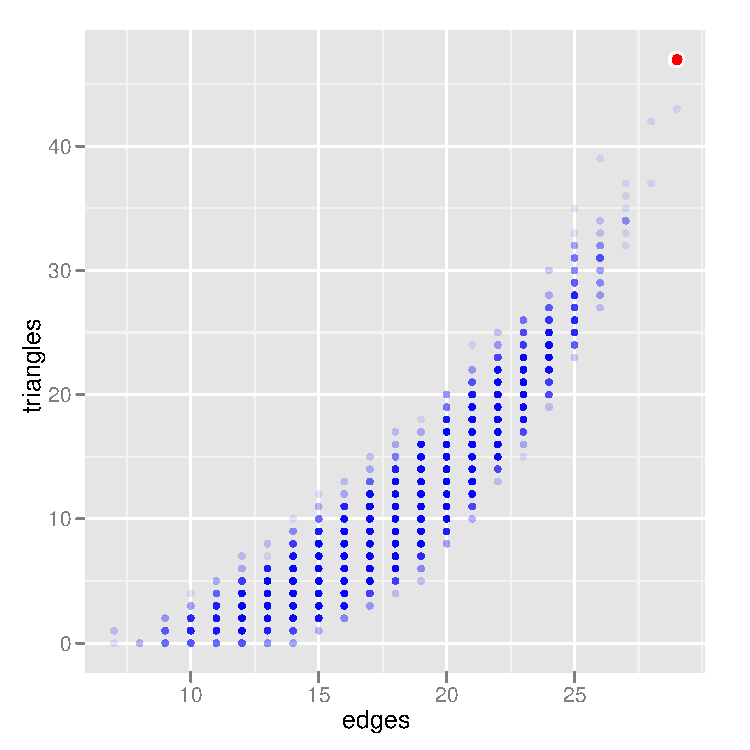
\includegraphics[width=\textwidth]{MCsample-bare} }}
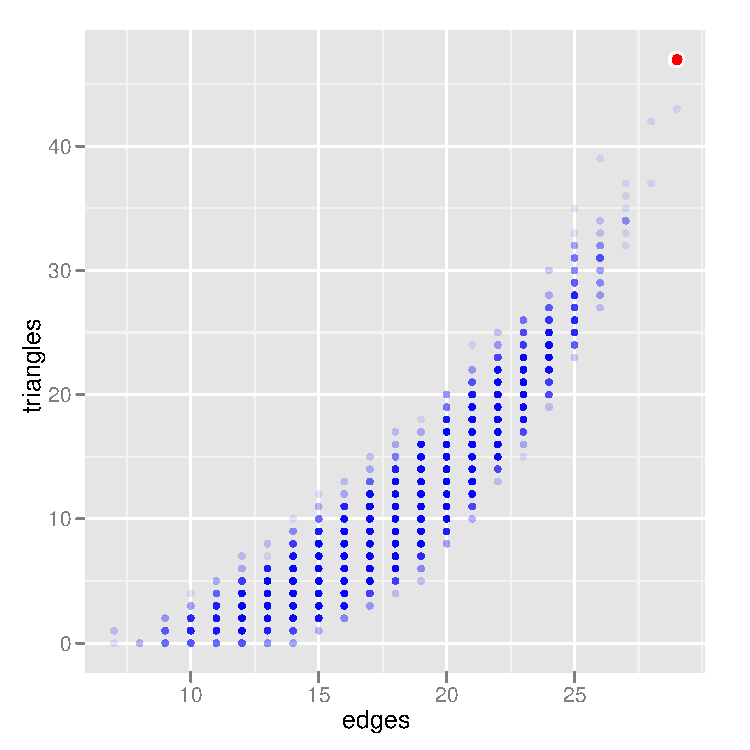
\includegraphics[width=2.15in]{MCsample-bare}
\end{column}

\begin{column}[r]{0.61\textwidth}
\pause

\begin{itemize}
\item But that's all we needed to find MLE before! 
\vspace{1mm}


\item Iterated samples %from distribution with parameter $\eta_k$ 
until %$\nabla \ell(\eta_k) = 0$, or
\begin{align*}
	\E_{\eta_k} g(Y) = g(\yobs).
\end{align*}

\end{itemize}
\end{column}
\end{columns}
}

\frame
{
\frametitle{Case: MLE exists}  
\begin{figure}[h]
\centering
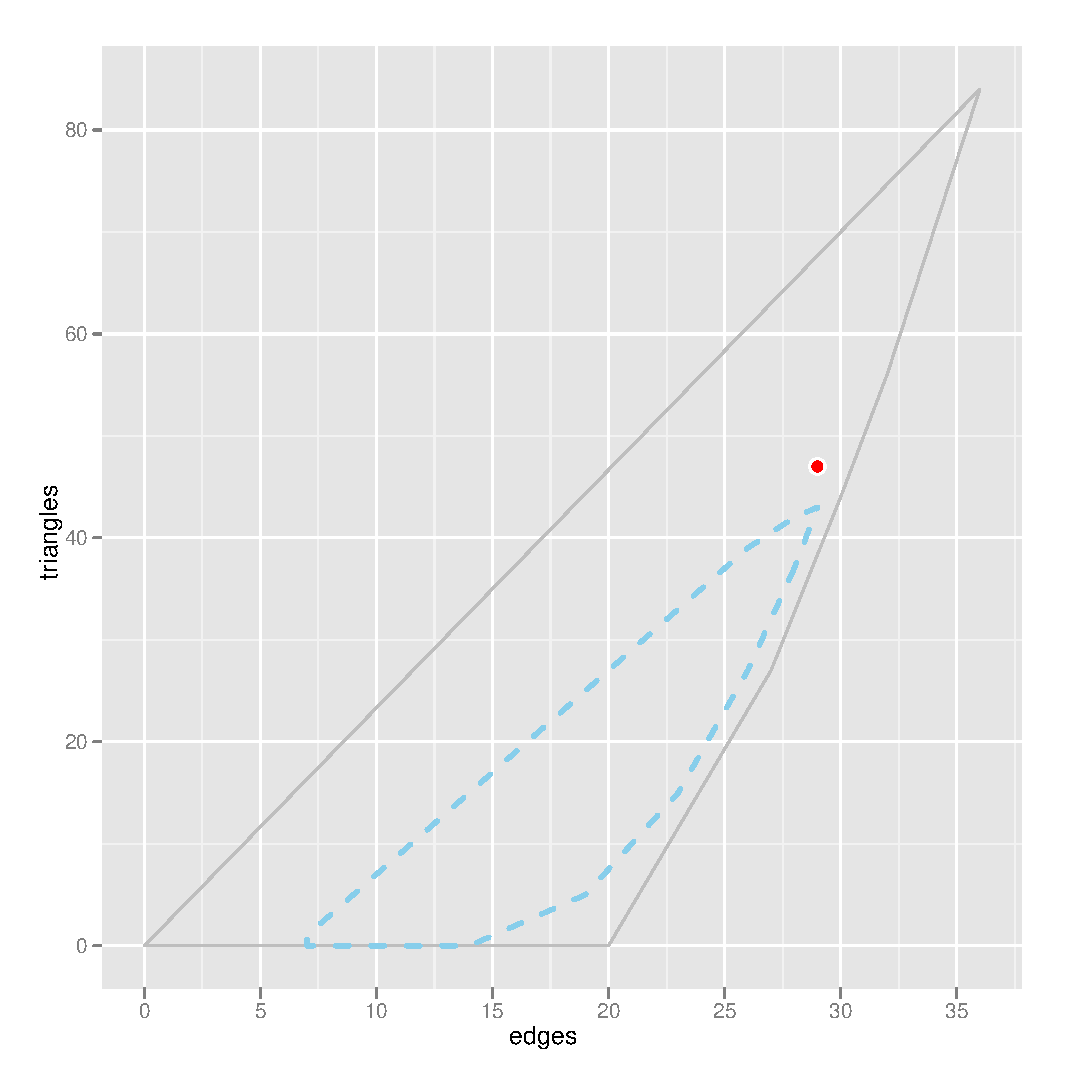
\includegraphics[height=2.2in]{MCsample-far}
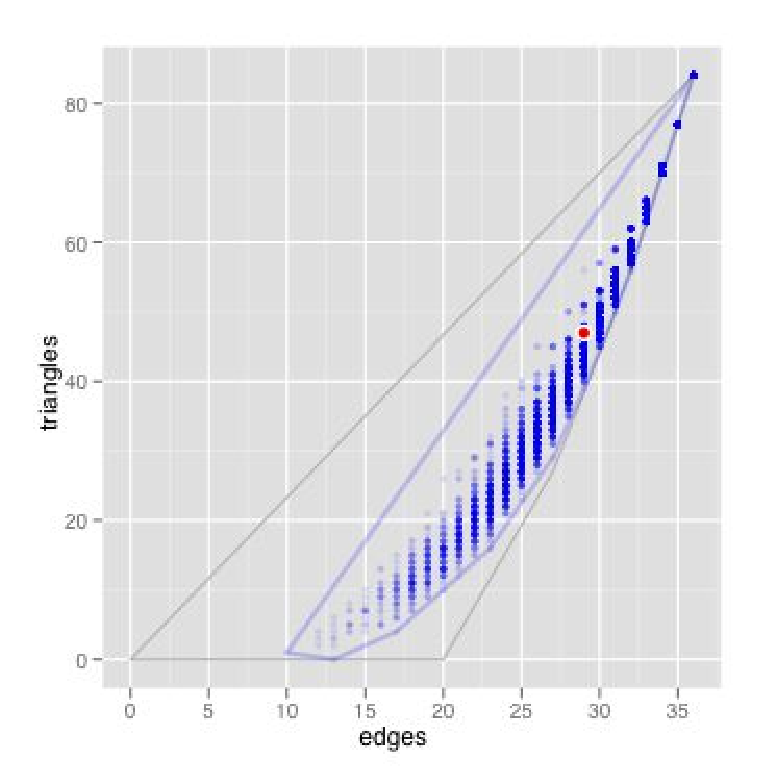
\includegraphics[height=2.2in]{MCsample-MLE}
\caption{MCMC samples from distributions with $\eta = (0,0)$ (left), and $\eta=\etaMLE$ (right).}
\label{F:MCsample-MLE exists}
\end{figure}
%MCMC samples from distributions with $\eta = (0,0)$ (left), and $\eta=\etaMLE$ (right).
}


\frame
{
\frametitle{Case: MLE does not exist}  
\begin{figure}[h]
\centering
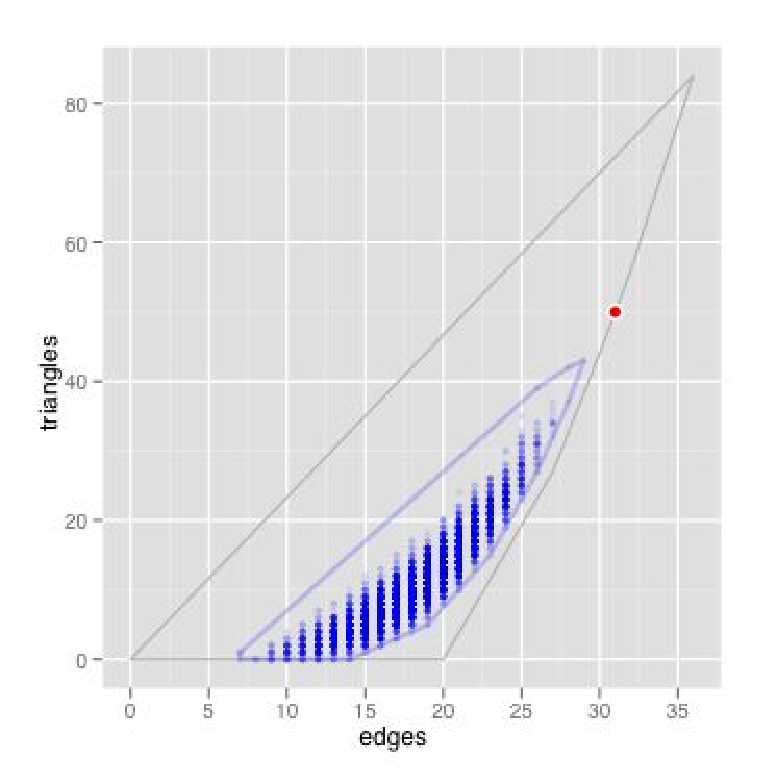
\includegraphics[height=2.2in]{MCsample-boundary}
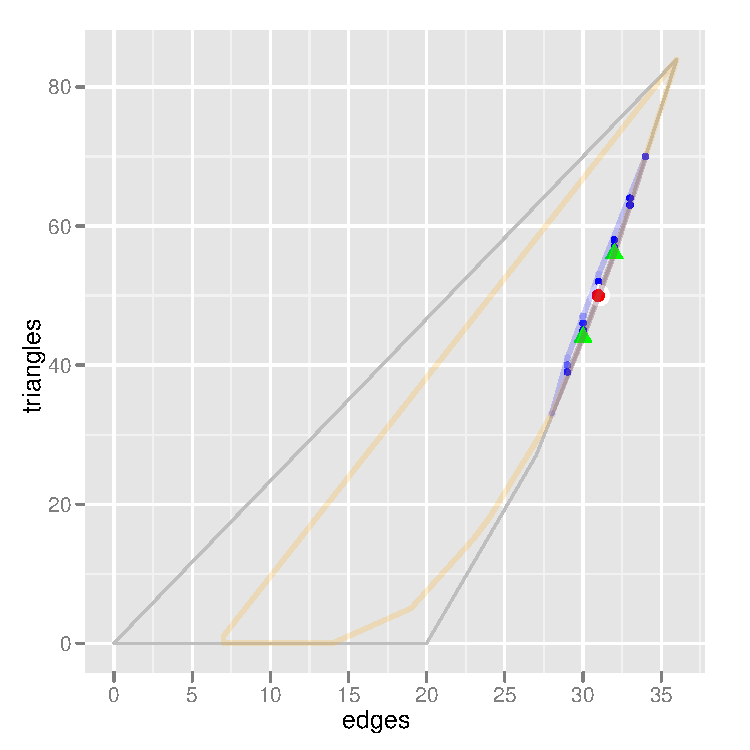
\includegraphics[height=2.2in]{MCsample-77face}
%\caption{MCMC samples from distributions with $\eta = (0,0)$ (left), and 
%when $\eta$ is close to MLE in LCM (right).}
\label{F:MCsample-MLE nonexistent}
\end{figure}
\pause
\emph{``I am transparent. You can see and feel me, but you cannot hold me. I always take the shape of my container. Who am I?"}
}
%\frame
%{
%\frametitle{Extending our algorithm}  
%%\setbeamercovered{transparent}
%\textbf{Idea}: Use MCMC samples to explore space and
%determine geometry of $C$.
%\vspace{2mm}
%
%Find a way to determine if
%\begin{enumerate}
%\item $g(\yobs)$ is on the boundary of our sample hull.
%
%\begin{figure}[h]
%\centering
%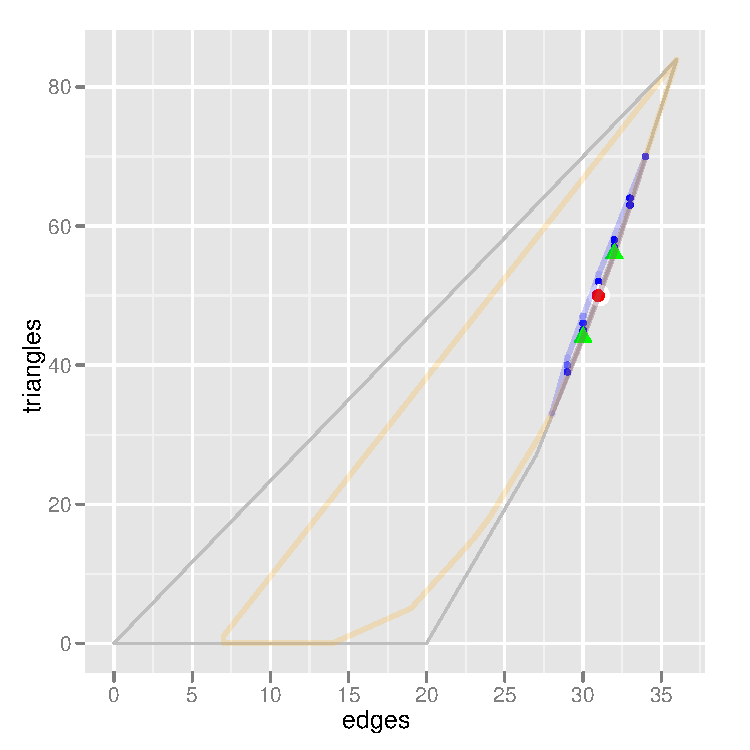
\includegraphics[height=1.5in]{MCsample-77face}
%\includegraphics[height=1.5in]{MCsample-interiorptonF}
%%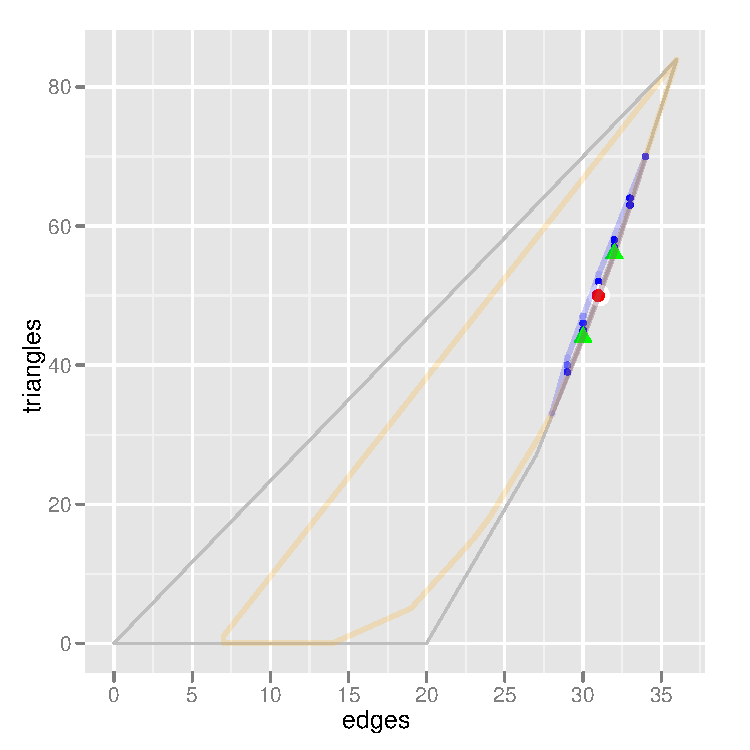
\includegraphics[height=2.2in, trim=3.5in 2in 0.in 0.0in, clip = true ]{MCsample-77face}
%%\includegraphics[height=2.2in, trim=2in 2in 0.in 0in, clip = true ]{MCsample-interiorptonF}
%%\caption{MCMC samples from distributions with $\eta = (0,0)$ (left), and 
%%when $\eta$ is close to MLE in LCM (right).}
%%\label{F:MCsample-MLE nonexistent}
%\end{figure}
%
%%\begin{columns}[]
%%\begin{column}[T]{0.25\textwidth}
%%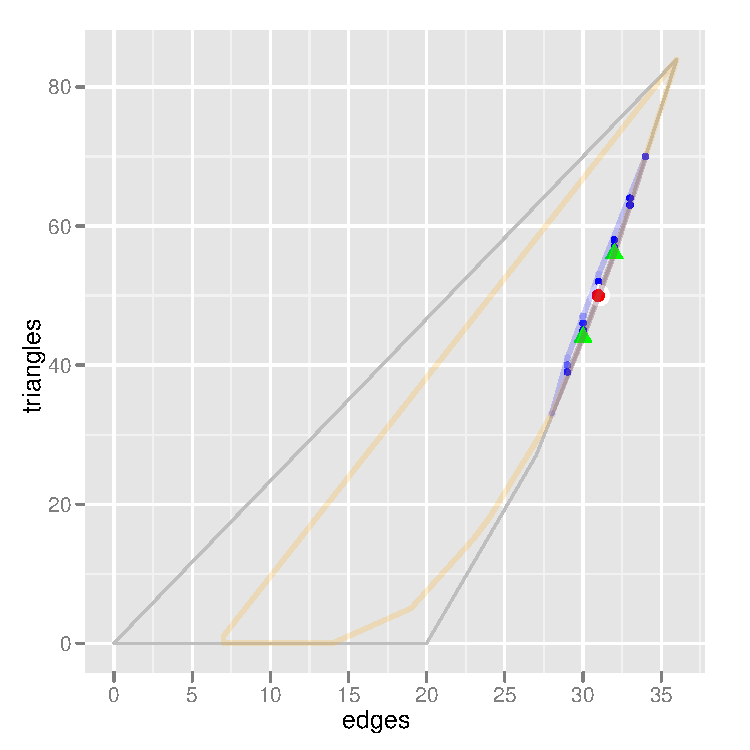
\includegraphics[height=2.5in,trim=3.5in 2in 0.15in 0.05in,clip=true]{MCsample-77face} % l b r t
%%\end{column}
%%\begin{column}[T]{0.25\textwidth}
%%\includegraphics[height=2.5in,trim=3.in 2in 0.15in 0.05in,clip=true]{MCsample-interiorptonF} % l b r t
%%\end{column}
%%\end{columns}
%}

\section{Algorithm extended: Issues}
\frame
{
\frametitle{Extending our algorithm}  
%\setbeamercovered{transparent}

\textcolor{darkblue}{Idea}: Use MCMC samples to explore space and determine geometry of $C$.
\begin{columns}[]
\begin{column}[T]{0.23\textwidth}
\begin{figure}[h]
\centering
\includegraphics[height=1.3in, trim=2.5in 1in 1in 1.9in, clip = true ]{MCsample-interiorptonF} % l b r t
\end{figure}
\end{column}

\begin{column}[t]{0.77\textwidth}
%\pause

\begin{enumerate}
\item Determine if $g(\yobs)$ is on boundary of sample hull.
\vspace{1mm}
\item If so, on what face \textcolor{blue}{$\tilde{F}$} \emph{of our sample hull}?
\vspace{1mm}
\item Find an empirical GDOR \textcolor{blue}{$\tilde{\delta}$} to \textcolor{blue}{$\tilde{F}$}.   
\end{enumerate}
\vspace{1mm}
These are problems in \textcolor{darkblue}{computational geometry}.  \\
Use tools in \textcolor{darkblue}{\texttt{rcdd}} package (Geyer and Meeden, 2009) based on Fukuda (2005).
\end{column}
\end{columns}
\vspace{2mm}

\pause

\begin{block}{Is \textcolor{blue}{$\tilde{F}$} also on boundary of $C$?}  
%That is, is $\tilde{F} = \alert{F}$?}
\vspace{1mm}

%\pause
\textcolor{darkblue}{Our approach:}

\textcolor{darkblue}{If} $>60\%$ of samples land on empirical \textcolor{blue}{$\tilde{F}$} 
\textcolor{darkblue}{then}\\
\hspace{2mm} \textcolor{blue}{$\tilde{F}$} is on boundary of $C$ \\
\textcolor{darkblue}{else} \\
\hspace{2mm} keep truckin'
\end{block}
}




\section{Algorithm extended: LCM}
\frame
{
\frametitle{Got 77\%.  One sided CI?}  
\begin{columns}[]
\begin{column}[T]{0.2\textwidth}
\centering
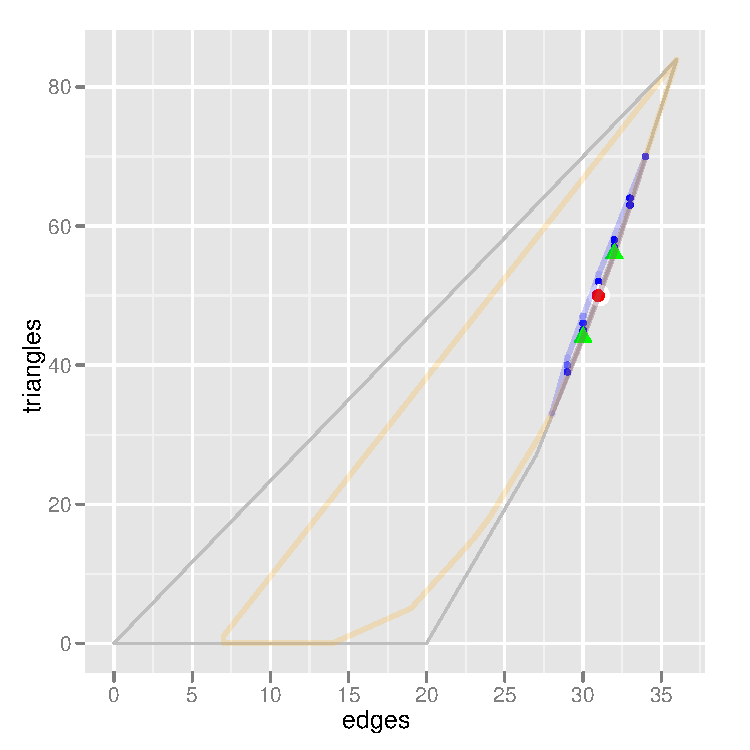
\includegraphics[ height=1.1in, trim=3.55in 2.1in 0.4in 0.9in, clip = true ]{MCsample-77face}
\end{column}
\begin{column}[T]{0.8\textwidth}
\textcolor{darkblue}{ More than 60\% of sample falls on \textcolor{blue}{$\tilde{F}$}.  Then}
\begin{enumerate}
\item \textcolor{blue}{$\tilde{F}$} is on boundary of $C$. %, \textcolor{blue}{$\tilde{F} = \alert{F}$}.
\item MLE does not exist (\alert{\checkmark}).
\item Empirical \textcolor{blue}{$\tilde{\delta}$} is a GDOR $\delta$ (\alert{\checkmark}).
\end{enumerate}
\vspace{1mm}

\textcolor{darkblue}{Still need MLE $\etaLCM$ for LCM.}
\end{column}
\end{columns}
\vspace{1mm}
\pause

But \textcolor{blue}{$\tilde{F}$} is the support for LCM
$\implies$ Use our algorithm to find $\etaLCM$!   (\alert{\checkmark})!
\vspace{5mm}

\pause
%\begin{align*}
%	\etaLCM = (126.8, -21.1)
%\end{align*}

\textcolor{darkblue}{Finally, one-sided CI for how close $\eta$ is to infinity.}  
\vspace{1mm}

%Find $\hat{s}$ such that $P_{\etaLCM + \hat{s} \delta}(\fatdot )$
%assigns probability $\alpha$ to $F$.

Find $\hat{s}$ for $\alpha$,
\begin{align*}
%\left [ \etaLCM + \hat{s} \delta, + \infty \right )
\left [ \left(\begin{array}{c}120.5 \\-20.06\end{array}\right) + \hat{s} \left(\begin{array}{r}6 \\-1\end{array}\right), + \infty \right )
\end{align*}
is a $1- \alpha$ confidence interval for the parameter $\eta^T\delta$.

%In this example,  
%\begin{align*}
%	[9.145, +\infty) \\
%	(-\infty, -1.500].
%\end{align*}
}


\section{Stacks}
\frame
{
\frametitle{Zooming out}  
\transboxin

\begin{center}
{\TINY \textcolor{blue}{one-sided CI}}

\uncover<2->{\scriptsize \textcolor{blue}{LCM MLE distribution}}

\uncover<3->{\small \textcolor{blue}{MLE non-existence}}

\uncover<4->{\normalsize \textcolor{blue}{parameter estimation}}

\uncover<5->{\large \textcolor{blue}{ERGMs}}

\uncover<6->{\Large \textcolor{blue}{discrete exponential families}}

\uncover<7->{\Huge \textcolor{blue}{ dependent data}}
%\only<1>{ \textcolor{blue}{dependent data}}
%\userbeamerfont{}{size=40pt} Saisuke
\end{center}
}


%%%%%%%%%%%%%%%%%%%%%%%%%%%%%%%%%%%%%%%%%%%%%%%%%%%%%%%%%%%%%%%%%%%%%%%%%%%%%%%%%%%%%%%%%%%%%%%%%%%%

\appendix
\newcounter{finalframe}
\setcounter{finalframe}{\value{framenumber}}


%%%%%%%%%%%%%%%%%%%%%%%%%%%%%%%%%%%%%%%%%%%%%%%%%%%%%%
\section{Reserve slides}

%\section{One-sided CI}
\frame
{
\frametitle{Visualizing a one-sided confidence interval}  
\begin{columns}[]
\begin{column}[T]{0.36\textwidth}
%\pause
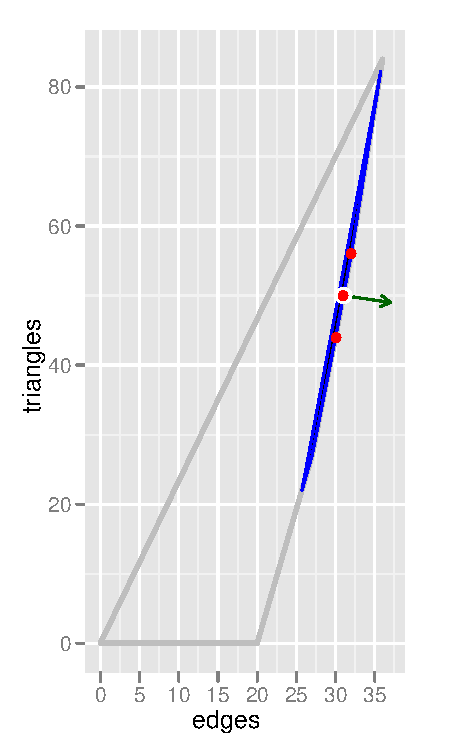
\includegraphics[height=3.3in,  trim=0.1in 0in 0.2in 0in, clip=True]{CI99-muspace} % l b r t
\end{column}

\begin{column}[t]{0.64\textwidth}

\textcolor{darkblue}{Mean value parameterization}

For a natural parameter $\eta$, the \textcolor{darkblue}{mean parameter $\mu$} is
\begin{align*}
	\mu = \E_\eta g(Y).
\end{align*}

%More interpretable because it's values are in $C$.
\vspace{2mm}

A conservative 99\% confidence region for $\mu$ 
can be overlaid on $C$.
\end{column}

\end{columns}
}

%\frame
%{
%\frametitle{When is our boundary \emph{the} boundary?}  
%\setbeamercovered{transparent}
%
%%\uncover<2->{
%
%\textcolor{darkblue}{Our approach} 
%
%If $>60\%$ of samples land on empirical $\tilde{F} \implies \tilde{F}$ is on boundary of $C$.
%
%Otherwise, keep sampling.
%%}
%\vspace{1mm}
%
%\begin{columns}[]
%\begin{column}[T]{0.22\textwidth}
%%\begin{figure}[h]
%\centering
%\includegraphics[width = 0.8in, height=1.2in, trim=3.5in 1.9in 0.3in 0.5in, clip = true ]{MCsample-77face} % l b r t
%%\caption{Two sample hulls with different $g(\yobs)$.}
%%\end{figure}
%\end{column}
%
%\begin{column}[t]{0.78\textwidth}
%
%%\pause
%%\textbf{First case}
%\textcolor{darkblue}{Case: $g(\yobs)$ on boundary}
%\begin{itemize}
%\item 77\% of samples fall on three points that define $\tilde{F}$.
%\item Conclude (correctly) that $\tilde{F}$ is on boundary of $C$, $\tilde{F} = \alert{F}$.
%\begin{itemize}
%\item MLE does not exist (\alert{\checkmark}).
%\item $\tilde{\delta}$ is a GDOR $\delta$ (\alert{\checkmark}).
%\end{itemize}
%\end{itemize}
%%\vspace{5mm}
%
%\end{column}
%\end{columns}
%\vspace{5mm}
%
%\begin{columns}[]
%\begin{column}[T]{0.22\textwidth}
%%\begin{figure}[h]
%\centering
%%\raggedright
%%\includegraphics[height=1.2in, trim=3.in 2in 0.15in 0.0in, clip = true ]{MCsample-interiorptonF}
%\includegraphics[width = 0.8in, height=1.2in, trim=2.9in 0.9in 0.9in 1.5in, clip = true ]{MCsample-interiorptonF} % l b r t
%
%%\includegraphics[width=.8in, height=1.2in, trim=2.5in 1in 1in 1.9in, clip = true ]{MCsample-interiorptonF} % l b r t
%
%%\caption{Two sample hulls with different $g(\yobs)$.}
%%\end{figure}
%\end{column}
%
%\begin{column}[t]{0.78\textwidth}
%
%%\pause
%%\textbf{Second case} 
%\textcolor{darkblue}{Case: $g(\yobs)$ in interior}
%\begin{itemize}
%\item 0.0001\% (1 point) falls on $\tilde{F}$.
%\item  Keep on truckin'.
%\end{itemize}
%\end{column}
%
%\end{columns}
%
%%\end{column}
%%\end{columns}
%}



\frame
{
\frametitle{Case: MLE exists, but observed data close to boundary}  
Observed data is $(21,4)$, in interior of $C$.
\begin{figure}[h]
\centering
\includegraphics[height=2.2in]{MCsample-problem}
\includegraphics[height=2.2in]{MCsample-fakeface}
\end{figure}
It is possible for all 10,000 MC samples to fall on empirical $\tilde{F}$, which is \textbf{not} on
$C$.
}


%\frame
%{
%\frametitle{Geometrically weighted edgewise shared partner (GWESP)}
%
%}

%\section{Algorithm: pseudocode}
\frame
{
\frametitle{Algorithm outline}
\setbeamercovered{transparent}
\small

Get an initial value, $\eta_0$.\\ 
Set $k=0$. \\
Set $p_0 = \nabla \ell( \eta_0)$, the direction of steepest ascent. \\
\vspace*{2mm}

\textbf{while}  $\lVert \nabla \ell( \eta_k) \rVert > \epsilon$ \\ 
\vspace*{1mm}

%\uncover<2->{
\hspace*{4mm} Find \alert{$\alpha_k$} that satisfies the 
\textcolor{darkblue}{curvature condition}
\begin{align*}
	 0 & \leq \nabla \ell( \eta_k + \alert{\alpha_k} p_k)^T p_k \leq c \nabla \ell(\eta_k)^T p_k
\end{align*}
\hspace*{4mm} \indent for some fixed $0 < c < 1$.  
\vspace*{1mm}
%} 

%\uncover<3->{
\hspace*{4mm} $\eta_{k+1} = \eta_k + \alert{\alpha_k} p_k$\\
%}
\vspace*{1mm}

%\uncover<5->{
\hspace*{4mm} $\nabla \ell( \eta_{k+1}) = g( y _{obs}) - \E_{\eta_{k+1}}g(Y)$\\
\vspace*{1mm}
 

\hspace*{4mm} \indent Find \alert{$p_{k+1}$}, which must be an ascent direction. \\


\hspace*{4mm} \indent $k = k + 1$  \\
%}

\textbf{end(while)}
}


%\frame
%{
%\frametitle{Next steps.}
%%Thoughts
%%\begin{itemize}
%%	\item Parameter is an index to a distribution.  Goal is the MLE distribution, not the number.
%%\end{itemize}
%
%Line search algorithm efficiency:
%\begin{itemize}
%	\item Switch criteria to MCMC-MLE or Newton-Raphson.  
%	\item Step size $\alpha_k$ search for curvature condition.
%%	\item Proof of convergence for noisy $\nabla \ell( \eta)$.
%\end{itemize}
%\vspace{2mm}
%
%When MLE does not exist, can do more with LCM MLE distribution.  In particular, hypothesis testing.
%}


%\frame
%{
%%\setbeamercovered{transparent}
%\frametitle{What is a one-sided CI}  
%
%Although $\ell(\eta)$ has no maximizer, it is bounded above by $\ell_{LCM}(\eta)$,
%which itself has a maximizer, $\etaLCM$.
%
%As $s \to +\infty$, $\ell(\eta + s \delta)$ converges to a point in LCM.
%The point $\ell(\etaLCM + s \delta)$ converges to $\sup_\eta \ell(\eta)$.
%
%Find unique $\hat{s}$ such that
%\begin{align*}
%		P_{\etaLCM + \hat{s} \delta}( g(Y) \in H) = \alpha.
%\end{align*}
%
%Then a $1- \alpha$ confidence interval for $s$ is 
%\begin{align*}
%[ \hat{s}, + \infty).
%\end{align*}
%
%In turn,
%\begin{align*}
%[ \etaLCM + \hat{s} \delta, + \infty)
%\end{align*}
%is a $1-\alpha$ CI for $\etaLCM + s \delta$.  
%%The values for $\eta$ that fall
%%in the region are in the neighborhood of the LCM MLE distribution.
%
%}

%\frame
%{
%%\setbeamercovered{transparent}
%\frametitle{\texttt{rcdd}}  
%
%\begin{columns}[]
%\begin{column}[T]{0.25\textwidth}
%\includegraphics[height=2.5in,trim=3.5in 2in 0.15in 0.05in,clip=true]{MCsample-77face} % l b r t
%\end{column}
%
%\begin{column}[T]{0.75\textwidth}
%\begin{enumerate}
%\item $g(\yobs) \notin$ sample hull.  
%
%%\uncover<2->{
%\textcolor{darkblue}{Check for existence of a strongly separating hyperplane using \texttt{lpcdd} function.}
%%}
%\vspace{2mm}
%
%\item Find face $\tilde{F}$ \emph{of sample hull} on which $g(\yobs)$ lies.  
%
%%\uncover<3->{
%\textcolor{darkblue}{Use \texttt{linearity} function.}
%%}
%\vspace{2mm}
%
%\item Find a GDOR $\tilde{\delta}$ orthogonal to $\tilde{F}$.  
%
%%\uncover<4->{
%\textcolor{darkblue}{Solve a linear programming problem
%using \texttt{lpcdd} to return a $\tilde{\delta}$.  }
%
%\textcolor{darkblue}{Here, $\tilde{\delta} = (6,-1)$.}
%%}
%\vspace{2mm}
%
%\item Determine if $\tilde{F}$ is also on boundary of $C$.  
%
%%\uncover<5->{
%\textcolor{blue}{Actually, \texttt{rcdd} doesn't give us this.}  
%%}
%\end{enumerate}
%\vspace{3mm}
%
%%\uncover<6->{
%\emph{Can do 1 -- 3 using rational arithmetic and without calculating expensive H-representations of hulls.}
%%}
%\end{column}
%\end{columns}
%}


\setcounter{framenumber}{\value{finalframe}}
\end{document}
